\documentclass{article}

% Recommended, but optional, packages for figures and better typesetting:
\usepackage{microtype}
\usepackage{graphicx}
\usepackage{subfig}
\usepackage{hyperref}

\usepackage{subcaption}
\usepackage{caption}
\captionsetup{font=small, labelfont=bf}
%\captionsetup[sub]{labelsep=period, subrefformat=brace}
%%%% Graphical Model code
\usepackage{tikz}

\usetikzlibrary{shapes.geometric, arrows}

\tikzset{
    latent/.style={circle, draw=white, thick, minimum size=1cm, fill={rgb,255:red,235; green,243; blue,251}},
    observed/.style={circle, draw=black, thick, minimum size=1cm},
    data/.style={circle, draw=white, thick, minimum size=1cm, fill={rgb,255:red,225; green,225; blue,225}},
    dashed_arrow/.style={-stealth, dashed, thick},
    solid_arrow/.style={-stealth, thick},
}
%%%%%%%%%%%
\usepackage{booktabs} % for professional tables
\newcommand{\theHalgorithm}{\arabic{algorithm}}
\newcommand{\norm}[1]{\left\lVert #1 \right\rVert_2}



% Use the following line for the initial blind version submitted for review:
\usepackage[accepted]{style/icml2025}

% If accepted, instead use the following line for the camera-ready submission:
% \usepackage[accepted]{style/icml2025}

% For theorems and such
\usepackage{hyperref}
\usepackage{amsmath}
\usepackage{amssymb}
\usepackage{bbm}
\usepackage{mathtools}
\usepackage{amsthm}
\usepackage{amsfonts}
\usepackage{amstext}
\usepackage{bm}
\usepackage{multirow}
\usepackage{relsize}
\usepackage{makecell}
\usepackage[flushleft]{threeparttable}
\usepackage{pdflscape}


\DeclareMathOperator*{\argminA}{arg\,min} 

% if you use cleveref..
\usepackage[capitalize,noabbrev]{cleveref}

%%%%%%%%%%%%%%%%%%%%%%%%%%%%%%%%
% THEOREMS
%%%%%%%%%%%%%%%%%%%%%%%%%%%%%%%%
\theoremstyle{plain}
\newtheorem{theorem}{Theorem}[section]
\newtheorem{proposition}[theorem]{Proposition}
\newtheorem{lemma}[theorem]{Lemma}
\newtheorem{corollary}[theorem]{Corollary}
\theoremstyle{definition}
\newtheorem{definition}[theorem]{Definition}
\newtheorem{assumption}[theorem]{Assumption}
\theoremstyle{remark}
\newtheorem{remark}[theorem]{Remark}
\newtheorem{example}[theorem]{Example}
\usepackage[textsize=tiny]{todonotes}

% \usepackage[numbers]{natbib}  % Use numeric style ??????



% The \icmltitle you define below is probably too long as a header.
% Therefore, a short form for the running title is supplied here:
\icmltitlerunning{}

% \usepackage{xcolor}
% \usepackage{relsize}
% \usepackage{multirow}
% \usepackage{bbm}
% \usepackage{todonotes}
%\usepackage{refcheck}
% \usepackage{algorithm}
% \usepackage{algpseudocode}
% \usepackage[hidelinks]{hyperref}
% \usepackage{appendix}
% \usepackage{amsthm}
% \usepackage{booktabs} % For professional table rules
% \usepackage{array}    % For better column alignment
% \usepackage{tikz}
% \usetikzlibrary{arrows.meta, shapes.geometric, positioning}
% \usetikzlibrary{bayesnet}
% % Define theorem environments
% \newtheorem{theorem}{Theorem}[section] % Theorem numbering follows section numbering
% \newtheorem{lemma}[theorem]{Lemma}     % Lemma shares numbering with Theorem
% \newtheorem{proposition}[theorem]{Proposition}
% \newtheorem{corollary}[theorem]{Corollary}
% \newtheorem{assumption}{Assumption}
% % Define a non-numbered environment for remarks and definitions
% \theoremstyle{definition}
% \newtheorem{definition}{Definition}[section]
% \newtheorem{remark}{Remark}[section]


\newcommand{\JOBID}{250106-prior_mnist_likelihood_poisson_model_unet_ep_20000_bs_200_slr_0.0001_ilr_0.00001_nhs_64}

\begin{document}

\twocolumn[
\icmltitle{Diffusion Models for Inverse Problems in the Exponential Family}

\icmlsetsymbol{equal}{*}

\begin{icmlauthorlist}
\icmlauthor{Alessandro Micheli}{equal,yyy}
\icmlauthor{Mélodie Monod}{equal,yyy}
\icmlauthor{Samir Bhatt}{yyy,comp}
\end{icmlauthorlist}

\icmlaffiliation{yyy}{Imperial College London}
\icmlaffiliation{comp}{University of Copenhagen}

\icmlcorrespondingauthor{Alessandro Micheli}{a.micheli19@imperial.ac.uk}
\icmlcorrespondingauthor{Mélodie Monod}{melodie.monod18@imperial.ac.uk}

% KEYWORD TODO
\icmlkeywords{Machine Learning, ICML}

\vskip 0.3in
]

\printAffiliationsAndNotice{\icmlEqualContribution} 

\begin{abstract}
    \begin{abstract}  
Test time scaling is currently one of the most active research areas that shows promise after training time scaling has reached its limits.
Deep-thinking (DT) models are a class of recurrent models that can perform easy-to-hard generalization by assigning more compute to harder test samples.
However, due to their inability to determine the complexity of a test sample, DT models have to use a large amount of computation for both easy and hard test samples.
Excessive test time computation is wasteful and can cause the ``overthinking'' problem where more test time computation leads to worse results.
In this paper, we introduce a test time training method for determining the optimal amount of computation needed for each sample during test time.
We also propose Conv-LiGRU, a novel recurrent architecture for efficient and robust visual reasoning. 
Extensive experiments demonstrate that Conv-LiGRU is more stable than DT, effectively mitigates the ``overthinking'' phenomenon, and achieves superior accuracy.
\end{abstract}  
\end{abstract}



% \paragraph{TODO List}

% ALESSANDRO:
% \begin{itemize}
% \item address my comments in 3.4 -- waiting for your response
% \item address todo on footnote in appendix A
% \item Write appendix D 
% \item Did you do all the todos below?
% \item Do you want to address of all sam's comments?
% \end{itemize}

% TODOS
% \begin{itemize}
% \item write appendix about Hx0
% \item for every statement we make about the derivative of $\log p_{\mathbf{x}_{0}\vert\mathbf{x}_t}$, clarify that it has to be sufficiently differentiable.
% \item add convexity KL divergence for exponential family (fisher information matrix) because we minimize it
% \item review number of eqs (some number needs to gathered, other removed)
% \item hilight benefit compared to mcmc: no prior evaluation, just sampling + no proposal, this is not done yet and needs to be done in the related work
% \end{itemize}

% MELODIE
% \begin{itemize}
%     \item Write related work
%     \item Write experiments
%     \item Critically read Appendix~\ref{app-proofs} and Section 4.4
% \end{itemize}


\section{Introduction} \label{sec:introduction}
% Score-based diffusion models provide a powerful mechanism to generate new samples from complex distributions through a two-step process~\citep{song2021scorebased}. First, they learn the score of the data distribution, defined as the gradient of the log-probability density function, at every time step $t$ of the noise process. Second, using this score, they iteratively refine noisy inputs to generate new samples from the data distribution.


\begin{figure*}[ht!]
\centering
\includegraphics[width=\textwidth]{plots/figure_diffusion_30_Jan.pdf}
\caption{\textbf{Illustration of the approach using Diffusion Models for Inverse Problems in the Exponential Family.} By leveraging the posterior score $\nabla_{\mathbf{x}_t} p_{\mathbf{x}_t|\mathbf{y}}(\mathbf{x}_t|\mathbf{y})$, a reverse stochastic differential equation (SDE) can be solved to generate posterior samples of the latent variable $\mathbf{x}_0$ from noise. Posterior samples of the parameter $\boldsymbol{\theta}$ are obtained by applying a deterministic inverse link function. The prior score function, $\nabla_{\mathbf{x}_t} p_{\mathbf{x}_t}(\mathbf{x}_t)$, is estimated using a neural network, following established approaches. A novel method is introduced to estimate the likelihood score function, $\nabla_{\mathbf{x}_t} p_{\mathbf{y}|\mathbf{x}_t}(\mathbf{y}|\mathbf{x}_t)$, leveraging the \textit{evidence trick} in combination with amortized variational inference.  The Figure illustrates the inference of a spatially inhomogeneous Poisson process where the intensity is as intricate as an ImageNet image.}
\label{fig-intro-summary-figure}
\end{figure*}


Score-based diffusion models offer a powerful framework for generating new samples from complex data distributions through a two-step process~\citep{song2021scorebased}. First, the score of the data distribution is estimated by learning to denoise corrupted samples. Second, leveraging this learned score, the noisy inputs are iteratively refined to produce new samples that align with the data distribution.


This capability is particularly advantageous in solving inverse problems. Given access to noisy observations $\mathbf{y} \in \mathbb{R}^{d_y}$, we are interested in inferring a latent signal $\mathbf{x}_0 \in \mathbb{R}^{d_x}$ that generated the observations by sampling from the posterior distribution $p_{\mathbf{x}_0|\mathbf{y}}(\mathbf{x}_0|\mathbf{y})$.
Diffusion models do not require the prior distribution $p_{\mathbf{x}_0}(\mathbf{x}_0)$ to be analytically specified or explicitly parameterized, they rely only on the ability to sample from it.
Therefore, they can be trained to learn the score of highly complex prior distributions, for instance where $\mathbf{x}_0$ are images from ImageNet. 
This distinguishes them from traditional methods like Markov Chain Monte Carlo (MCMC), which necessitates evaluating the prior density.


Despite these advantages, current diffusion-based methodologies are predominantly confined to Gaussian likelihoods (e.g.,~\citet{kadkhodaie2021, kawar2021, kawar2022, chung2023, song2023pseudoinverseguided, boys2024, rozet2024}), limiting their applicability to scenarios such as image deblurring or denoising. 
However, many scientific applications involve likelihoods that deviate significantly from Gaussian distributions. For instance, event data (e.g., COVID-19 case counts) is naturally modeled using a Poisson distribution, while proportion data (e.g., prevalence rates) aligns with a Binomial distribution. 
% These deviations present significant challenges, as existing diffusion-based methods are ill-equipped to handle such complexities.

One major obstacle to extending diffusion models to non-Gaussian likelihoods lies in the intractability of the posterior distribution score at diffusion time $t$, $ p_{\mathbf{x}_t | \mathbf{y}}(\mathbf{x}_t | \mathbf{y})$. Specifically, the posterior distribution score incorporates both the the prior score at time $t$, $ p_{\mathbf{x}_t}(\mathbf{x}_t)$, which can be trained, and the likelihood score at time $t$, $p_{\mathbf{y} | \mathbf{x}_t }(\mathbf{y}| \mathbf{x}_t )$. 
The latter is generally intractable because it depends on an integral over the reverse diffusion process density, which is itself difficult to compute. 
A common approach, when the observations follow a Gaussian distribution, is to approximate the reverse diffusion process and derive a closed-form expression for the likelihood score.
This approach is used by methods like Diffusion Posterior Sampling (DPS)~\citep{chung2023}, which proposes a delta function approximation centered at the Tweedie's posterior first moment, and Tweedie Moment Projected Diffusions~\citep{boys2024}, which employed a Multivariate anisotropic Gaussian distribution approximation. 


These methods have significant limitations. They often struggle to accurately quantify uncertainty in the reverse diffusion process and they rely on Tweedie’s formula~\citep{Efron2011}, which exhibits high variance at high noise levels (see Section 1.2 of~\citet{target_score_matching}). 
Additionally, they cannot accommodate non-Gaussian observations. While~\citet{chung2023} proposed using Gaussian approximations for non-Gaussian distributions --- such as approximating a Poisson distribution with a Gaussian --- this approach is highly unstable for small values and entirely inapplicable to certain distributions.
These limitations underscore the need for robust methodologies that extend the applicability of diffusion models to non-Gaussian settings, ensuring both stability and accurate representation of diverse likelihoods.

To address these limitations, we introduce an approach that we term, the \textit{evidence trick}. By leveraging the properties of the exponential family and employing an amortized variational approach, we extend the applicability of diffusion models for inverse problems to any likelihood distribution within the one-parameter exponential family, which includes the Poisson and Binomial distributions. 
To approximate the likelihood score, $p_{\mathbf{y}|\mathbf{x}_t}(\mathbf{y}|\mathbf{x}_t)$, we use the conjugate prior distribution as a variational approximation for the reverse diffusion process. This reformulation makes the integral over the reverse process tractable and accounts for parameter uncertainty. In contrast to previous approaches, we derive an objective to optimize the variational distribution that is independent of the reverse process expectation, bypassing the need for Tweedie's formula. Figure~\ref{fig-intro-summary-figure} graphically summarises our methodology.


We leverage our methodology to introduce a \textit{``Score-Based Cox process''}, a discrete Cox process where the intensity is modeled using a score-based diffusion process. We demonstrate that our model can effectively capture rough and intricate intensity patterns, including those as complex as image samples from the ImageNet database. Furthermore, we show that our methodology can address real-world scientific challenges by performing competitively with the current state-of-the-art in predicting malaria prevalence estimates in Sub-Saharan Africa.

% In summary, this paper makes the following contributions:
% \begin{itemize}
%     \item We extend score-based diffusion models for inverse problem methodologies to distributions within the one-parameter exponential family (e.g., Poisson, Binomial), enabling their application to a wider range of scientific problems.
%     \item We demonstrate that there exists a variational distribution that can optimally approximate the reverse process through an objective function that is independent of expectations over the reverse process, thereby avoiding reliance on Tweedie’s formula.
% \end{itemize}



% To the best of our knowledge, no prior work has systematically addressed inverse problems with non-Gaussian likelihoods using diffusion models. The rest of this paper is organized as follows: [insert structure overview].



% diffusion model using score based, show equaion o the score
% diffusin model for inverse bayesian problem with equation of the score. the score of the prior and the score of the likelihood. 
% while it seems trighforwar dte score of the likelihood is not tractable because it depends on t. so you need to approximate it. 
% We can obtain sample from the posterior. And the keu difference with MCMC is that the priro should not have to be evaluated but only sampled from. With their flexibility, diffusion models replace handcrafted priors on the latent signal with pretrained and
% strong empirical priors. For example, given a latent signal x0 (say a face image), we can train a diffusion model to sample from the prior p(x0). . In other words, we could sample prior from images, which have an underlying complex probability distribution, but it does not have to be tractable to do inference with it. 
% current methodologies have heavly been focused on the gaussian likelihood case, ss it was applied to images debluring xxx , xx. However this methodlogies could be extended to more scienific problem msot of which do not have a gaussian lileihood. Thi could include event data (cases of COVID-19 in epidemiology) or proportion data (prevalence of COVID-19 in epiedemiogloy). These data are often mdoelling with a latent representation, either a gaussian process or splines. But these methods are prohbitive computational cost or flexibility. Additionaly they require to have a clost form prior. This methodology could allow to use represnetation of latent function where the prior is specified by images or other very complex distribution one can sample from, and could model the latent funciton of other type of data. In this paper we show that the methodology can be extended to any data for which the distibution belongs to the one parameter exponential family, this includes the poisson, binomial as well as the gaussian witha fixed variance. Note that in the preivous application, the gaussian had always a fixed variance as the latent function is always placed on the mean. In our best knowledge,  no other methodologies have been apploeid to a broader class of distirbution except if the distribution was approximated with a gaussian, for example Chung proposed an approach to use Poisson distirbuted data, however this considers the data as a gaussian approxiamation, which is incorrect for small poisson values. 


% This paper is devoted to developing novel methods to solving inverse problems, given a latent (target) signal x0 ∈ R
% dx , noisy observed data y ∈ R
% dy , a known linear observation map H, and a pretrained diffusion prior.

% the likelihodo dependent of the process can be shown to be an integral of the likelihood and the reverse sde process, which is untractbale. all methods proposed have proposed to employ a gaussian approximation on the reverse sde, which will be more detailed in the background. this gaussian approximation is then parametrized to be as close as possible to the true distirbution  relying on tweedie formula which can be highly unstabel because it is divided by alpha which is close to 0 near t. Instead we propose the evidence trick, which place the conjugate distirbution of the likelihood as a variation distribution and allow the integral to be available in close form. Then to match the best distribution with amortized variational inference by showing that the objective functin can be reduced to not be dependent on the untractable reverse process.



% Things we need to explain in the intro
% \begin{itemize}
% \item Why is it important to extend the current methodologies beyond the normal normal case?
% \item Why is it important to have parametric models (e.g. intensity based models) instead of fully non-parametric models (e.g. intensity free models)? 
% \end{itemize}
% We notice that Chung proposed an approach to use Poisson distirbuted data, however this considers the data as a gaussian approxiamation, which is incorrect for small poisson values.



\section{Background} \label{sec:background}
Throughout this work, vectors and matrices will be represented using boldface notation, denoted as $\mathbf{x}$, while scalars will be expressed in standard font as $x$. Furthermore, we will use $\norm{\mathbf{x}}$ to denote the $\ell^{2}$-norm of a vector $\mathbf{x}$.
\subsection{Score-Based Diffusion Models} 
\label{sec-score-based-diffusions}
Score-based diffusion models aim to generate samples from a target distribution $ p_{\mathbf{x}_0}(\mathbf{x}_0) $ by progressively perturbing data with increasing noise levels and then learning to reverse this perturbation. This reversal defines a generative model capable of approximating the original data distribution. In this work, we adopt the framework introduced by \citet{song2021scorebased}, who define the forward noising process via an Itô stochastic differential equation (SDE). Specifically, we focus on the Variance-Preserving (VP) formulation of the SDE presented by~\citet{song2021scorebased}, which corresponds to the Denoising Diffusion Probabilistic Models (DDPM) introduced by~\citet{ho_denoising}.

We construct a forward diffusion process $ (\mathbf{x}_t)_{t \in [0,T]} $, with $ \mathbf{x}_t \in \mathbb{R}^{d_x} $, governed by the following equation:
\begin{equation*}
\mathrm{d}\mathbf{x}_t = - \frac{1}{2} \beta(t) \mathbf{x}_t \, \mathrm{d}t + \sqrt{\beta(t)} \, \mathrm{d}\mathbf{w}_t, \quad \mathbf{x}_0 \sim p_{\mathbf{x}_0},
\end{equation*}
where $ \mathbf{w}_t $ denotes a standard Wiener process, and $ \beta(t) : \mathbb{R} \to \mathbb{R}_+$ is a noise schedule. A commonly chosen parametrization for the noise schedule is the linear schedule $ \beta(t) = \beta_0 + t \, (\beta_1 - \beta_0) $, as discussed in \citet[Appendix C]{song2021scorebased}. The forward process is associated with the following transition kernel:
\begin{equation}
\label{eq-forward-transition-kernel}
p_{\mathbf{x}_t | \mathbf{x}_0}(\mathbf{x}_t | \mathbf{x}_0) = \mathcal{N}(\mathbf{x}_t; \sqrt{\alpha_t} \mathbf{x}_0, v_t \mathbf{I}_{d_x}),
\end{equation}
where $ \alpha_t := \exp\left( - \int_0^t \beta(s) \, \mathrm{d}s \right) $ and $ v_t := 1 - \alpha_t $. 

To recover the data-generating distribution, we reverse the noising process by solving the reverse SDE, derived from the forward process \cite{anderson_1982}:
\begin{multline*}
\mathrm{d}\mathbf{x}_t = - \beta(t) \left( \frac{1}{2} \mathbf{x}_t + \nabla_{\mathbf{x}_t} \log p_{\mathbf{x}_{t}}(\mathbf{x}_t) \right) \, \mathrm{d}t   \\ + \sqrt{\beta(t)} \, \mathrm{d}\bar{\mathbf{w}}_t, \quad \mathbf{x}_T \sim p_{\mathbf{x}_T},
\end{multline*}
where $\mathrm{d}t$ corresponds to time running backward, $\mathrm{d}\bar{\mathbf{w}}_t$ to the standard Wiener process running backward. Importantly, the term $ \nabla_{\mathbf{x}_t} \log p_{\mathbf{x}_{t}}(\mathbf{x}_t) $ is the score function, which guides the reverse process and it is typically approximated using a neural network $ \mathbf{s}_{\boldsymbol{\phi}}$, with learnable parameters $\boldsymbol{\phi}$, trained via Denoising Score Matching (DSM)~\cite{vincent2011} using the objective
\begin{multline}\label{eq:phi_star}
    \mathcal{J}_{\text{DSM}}(\boldsymbol{\phi}) =\\  \mathbb{E}_{t\sim U(\epsilon, 1)}\Big[ \lambda(t)  \mathbb{E}_{ \mathbf{x}_0\sim  p_{\mathbf{x}_0}, \mathbf{x}_t \sim p_{\mathbf{x}_t\vert\mathbf{x}_0}}\Big[ \mathcal{L}_{\text{DSM}}(\boldsymbol{\phi},  \mathbf{x}_0, \mathbf{x}_t, t)\Big]\Big], 
\end{multline}
with 
\begin{multline*}
\mathcal{L}_{\text{DSM}}(\boldsymbol{\phi}, \mathbf{x}_0, \mathbf{x}_t, t) = \\  \norm{\mathbf{s}_{\boldsymbol{\phi}}(\mathbf{x}_t, t) 
    -  \nabla_{\mathbf{x}_t} \log p_{\mathbf{x}_t\vert\mathbf{x}_0}(\mathbf{x}_t\vert\mathbf{x}_0)}^2,
\end{multline*}
and where $\epsilon \approx 0$ is a small positive constant, $\lambda(t) :[0,T]\to\mathbb{R}_+$ is a positive weighting function typically set to $\lambda(t) = 1/ \mathbb{E}\left[\left\vert\left\vert\nabla_{\mathbf{x}_t} \log p_{\mathbf{x}_t\vert\mathbf{x}_0}(\mathbf{x}_t|\mathbf{x}_0) \right\vert\right\vert_2^2\right]$ (see~\citet[Section 3.3]{song2021scorebased}). Once $\boldsymbol{\phi}^{*}$ is acquired by minimizing~\eqref{eq:phi_star}, one can use the approximation $\nabla_{\mathbf{x}_t} \log p_{\mathbf{x}_t}(\mathbf{x}_t) \simeq \mathbf{s}_{\boldsymbol{\phi}^*}(\mathbf{x}_t, t)$. 

\subsection{Inverse Problems with Diffusion Models}
\label{sec-diffusion-posterior-sampling}

Inverse problems across various scientific domains share a unified mathematical framework. The objective in these problems is to infer unknown parameters $\mathbf{x}_{0}$ given a set of measurements 
$\mathbf{y} \in \mathbb{R}^{d_{y}}$.
To solve such problems in a Bayesian framework, one adopts a prior distribution $p_{\mathbf{x}_0}(\mathbf{x}_0)$ and a likelihood distribution  $p_{\mathbf{y}|\mathbf{x}_0}(\mathbf{y}|\mathbf{x}_0)$, and seeks to sample from the posterior distribution $p_{\mathbf{x}_0|\mathbf{y}}(\mathbf{x}_0|\mathbf{y})$. 
Using Bayes’ rule, the posterior is given by:
\begin{equation*}
p_{\mathbf{x}_0|\mathbf{y}}(\mathbf{x}_0|\mathbf{y}) = \frac{ p_{\mathbf{y}|\mathbf{x}_0}(\mathbf{y}|\mathbf{x}_0)p_{\mathbf{x}_0}(\mathbf{x}_0)}{p_{\mathbf{y}}(\mathbf{y})},
\end{equation*}
where the \textit{evidence} is $p_{\mathbf{y}}(\mathbf{y}) = \int p_{\mathbf{y}|\mathbf{x}_0}(\mathbf{y}|\mathbf{x}_0)p_{\mathbf{x}_0}(\mathbf{x}_0) d\mathbf{x}_0$. The diffusion-based approaches of Section~\ref{sec-score-based-diffusions} can be adapted to sample from the posterior by adopting the following reverse process
\begin{multline}
\label{eq:reverse_SDE_posterior}
\mathrm{d}\mathbf{x}_t = - \beta(t) \left(\frac{1}{2}\mathbf{x}_t+ \nabla_{\mathbf{x}_t}\log p_{\mathbf{x}_{t}\vert \mathbf{y}}(\mathbf{x}_t|\mathbf{y})  
\right)  \mathrm{d}t \\ + \sqrt{\beta(t)} \mathrm{d}\bar{\mathbf{w}}_t, \quad \mathbf{x}_T \sim p_{\mathbf{x}_T|\mathbf{y}}. 
\end{multline}
It follows from Bayes' rule that the score of the posterior is 
\begin{multline} 
\label{eq:score_posterior}
    \nabla_{\mathbf{x}_t }\log p_{\mathbf{x}_t | \mathbf{y}}(\mathbf{x}_t | \mathbf{y}) = \\ \nabla_{\mathbf{x}_t } \log p_{\mathbf{x}_t}(\mathbf{x}_t) + \nabla_{\mathbf{x}_t } \log p_{\mathbf{y}|\mathbf{x}_t}(\mathbf{y}|\mathbf{x}_t).
\end{multline}
Hence, computing the score of the posterior distribution can be reduced to evaluating two terms: the prior score function, $\nabla_{\mathbf{x}_t }\log p_{\mathbf{x}_t}(\mathbf{x}_t)$, and the likelihood score function,$\nabla_{\mathbf{x}_t} \log p_{\mathbf{y}|\mathbf{x}_t}(\mathbf{y}|\mathbf{x}_t)$. The former can be directly obtained using the trained prior score function $\mathbf{s}_{\phi^*}(\mathbf{x}_t, t)$. However, computing the latter is challenging in closed form due to its dependence on time $t$, as there is only an explicit dependence between $\mathbf{y}$ and $\mathbf{x}_0$. To address this, \citet{chung2023} propose to factorize
$p_{\mathbf{y}|\mathbf{x}_t}(\mathbf{y}|\mathbf{x}_t )$ as:
\begin{equation}
\label{eq-likelihood-y-xt}
    p_{\mathbf{y}|\mathbf{x}_t}(\mathbf{y}|\mathbf{x}_t ) 
    = \int p_{\mathbf{y}|\mathbf{x}_0}(\mathbf{y}|\mathbf{x}_0) p_{\mathbf{x}_0|\mathbf{x}_t}(\mathbf{x}_0|\mathbf{x}_t) \mathrm{d}\mathbf{x}_0,
\end{equation} 
which follows from the fact that $\mathbf{y}$ and $\mathbf{x}_{t}$ are conditionally independent given $\mathbf{x}_{0}$. The density $p_{\mathbf{x}_0|\mathbf{x}_t}(\mathbf{x}_0|\mathbf{x}_t)$ is generally intractable, making the approximation of the integral in~\eqref{eq-likelihood-y-xt} a challenging task.


\subsection{Sampling for Linear Inverse Problems}
\label{sec-sampling-linear-inverse-problem}

The existing literature has predominantly focused on applications where observations follow a Gaussian likelihood:
\begin{equation*} 
%\label{eq:gaussian_gaussian_case}
    \mathbf{y} = \mathcal{H}( \mathbf{x}_0) + \mathbf{u}, \quad \text{where} \quad \mathbf{u} \sim \mathcal{N}(0, \sigma_y^2 \mathbf{I}_{d_y}),
\end{equation*}
where $\mathcal{H}:\mathbb{R}^{d_{x}}\to\mathbb{R}^{d_{y}}$ is the forward measurement operator and $\mathbf{u}$ is the measurement noise.
Practical applications relevant to this work often involve a potentially non-invertible linear setting, where $ \mathcal{H}(\mathbf{x}_0) = \mathbf{H}\mathbf{x}_0 $ for an $ d_{y} \times d_{x} $ real matrix $ \mathbf{H} $ with $ d_{x} \leq d_{y} $. In this context, existing studies~\cite{chung2023,song2023pseudoinverseguided, boys2024,rozet2024} approximate the integral in~\eqref{eq-likelihood-y-xt} by employing a Gaussian approximation, $ q_{\mathbf{x}_0|\mathbf{x}_t}(\mathbf{x}_0|\mathbf{x}_t) $, for the true posterior distribution $ p_{\mathbf{x}_0|\mathbf{x}_t}(\mathbf{x}_0|\mathbf{x}_t) $. This Gaussian approximation is defined as:  
\begin{equation*} %\label{eq:gaussian_variational_distribution}  
q_{\mathbf{x}_0|\mathbf{x}_t}(\mathbf{x}_0|\mathbf{x}_t) = \mathcal{N}_{d_x}(\mathbf{x}_0; \mathbf{m}_0(\mathbf{x}_t), C_0(\mathbf{x}_t)),  
\end{equation*}  
where $ \mathbf{m}_0(\mathbf{x}_t) $ and $ C_0(\mathbf{x}_t) $ are the mean and covariance of the approximation, respectively. This approach enables the computation of closed-form expressions for $ p_{\mathbf{y}|\mathbf{x}_t}(\mathbf{y}|\mathbf{x}_t) $, as the integral in Equation~\eqref{eq-likelihood-y-xt} becomes analytically tractable\footnote{We informally interpret the delta function approximation in \citet{chung2023} as a degenerate Gaussian distribution where the variance approaches zero.}. 

Relevant to our work is the approach adopted by \citet{boys2024} who proposed approximating $ p_{\mathbf{x}_0|\mathbf{x}_t}(\mathbf{x}_0|\mathbf{x}_t) $ by projecting it onto the closest Gaussian distribution $ q_{\mathbf{x}_0|\mathbf{x}_t}(\mathbf{x}_0|\mathbf{x}_t) $ in terms of the Kullback-Leibler (KL) divergence. The closest Gaussian in this sense is the one that matches the first two moments, $\mathbb{E}_{p_{\mathbf{x}_0|\mathbf{x}_t}}[\mathbf{x}_0]$ and $\mathbb{E}_{p_{\mathbf{x}_0|\mathbf{x}_t}}[\mathbf{x}_0 \mathbf{x}_0^\top]$,  of the true posterior distribution. They estimated these moments using Tweedie's formula~\cite{Efron2011}.  



\section{Sampling for Diffusion Models with Conjugacy Structure} \label{sec:method}

The results presented in this section are derived using the theoretical framework and properties of exponential family distributions, which are thoroughly reviewed in Appendix~\ref{app-exponential-family}. 
% The relevant assumptions underlying this framework are also discussed in detail in the appendix.

\subsection{Setup}
The dataset $\mathbf{y} = \{ \boldsymbol{y}_i \}_{i=1}^N$ is assumed to consist of $N$ independent and identically distributed (i.i.d.) observations. Each observation $\boldsymbol{y}_i \in \mathcal{Y}^d \subseteq \mathbb{R}^d$ is derived from a parameter vector $\boldsymbol{\theta} \in \Theta^d \subseteq \mathbb{R}^d$ through the conditional distribution $p_{\boldsymbol{y} \vert \boldsymbol{\theta}}(\boldsymbol{y}_i \vert \boldsymbol{\theta})$ for $i = 1, \ldots, N$. 
The components of $\boldsymbol{y}_i$ and $\boldsymbol{\theta}$ are denoted by $\boldsymbol{y}_i = (y_{i,1}, y_{i,2}, \ldots, y_{i,d})$ and $\boldsymbol{\theta} = (\theta_1, \theta_2, \ldots, \theta_d)$, respectively. 
Henceforth we will work under the following assumptions. 
\begin{assumption}[Conditional Independence of Variables]
\label{ass-independence-y}
The variable $y_{i,j}|\boldsymbol{\theta}$ is independent of $y_{i,k}|\boldsymbol{\theta}$ for all $j \neq k$ and for all $i = 1, \ldots, N$. Furthermore, we assume that $y_{i,j}| \theta_j$ is independent of $\theta_{k}$ for all $j \neq k$.
\end{assumption}
\begin{assumption}[Exponential Family Distribution]
\label{ass-exponential-distribution}
The distribution $p_{{y} \vert {\theta}}(y_{i,j} \vert {\theta}_j)$ belongs to the univariate one-parameter exponential family with natural parameter $\eta(\theta_j)$, base measure $h_{y}(y_{i,j})$, sufficient statistics $T_{y}(y_{i,j})$ and log-partition function $A_y(\eta(\theta_j))$ for $j = 1, \ldots, d$ and $i = 1, \ldots, N$.
\end{assumption}
Given Assumptions~\ref{ass-independence-y} and~\ref{ass-exponential-distribution}, it follows that the distribution $p_{\boldsymbol{y} \vert \boldsymbol{\theta}}(\boldsymbol{y}_i \vert \boldsymbol{\theta})$ belongs to the multivariate exponential family with the form
\begin{multline*}
p_{\boldsymbol{y}\vert\boldsymbol{\theta}}(\boldsymbol{y}_i \vert \boldsymbol{\theta}) =\\  h_{\boldsymbol{y}}(\boldsymbol{y}_i)   \exp \left( \boldsymbol{\eta}(\boldsymbol{\theta})^{\top} \mathbf{T}_{\boldsymbol{y}}(\boldsymbol{y}_i) - \mathbf{1}_d^\top \mathbf{A}_{\boldsymbol{y}}(\boldsymbol{\eta}(\boldsymbol{\theta})) \right),
\end{multline*}
for $i = 1, \ldots, N$ and where $\mathbf{1}_d$ is a vector of ones of dimension $d$ and
\begin{equation*}
\begin{aligned}
&h_{\boldsymbol{y}}(\boldsymbol{y}_i) = \prod_{j = 1}^d h_{y}\left(y_{i,j}\right), \\ 
&\boldsymbol{\eta}(\boldsymbol{\theta}) = \left(\eta(\theta_1), \dots, \eta(\theta_d)\right), \\
&\mathbf{T}_{\boldsymbol{y}}(\boldsymbol{y}_i) = \left(T_y(y_{i,1}), \ldots, T_y(y_{i,d})\right), \\
&\mathbf{A}_{\boldsymbol{y}}\left(\boldsymbol{\eta}\left(\boldsymbol{\theta}\right)\right) = \left(A_y\left(\eta\left(\theta_1\right)\right), \ldots, A_y\left(\eta\left(\theta_d\right)\right)\right).
\end{aligned}
\end{equation*}
Furthermore, since 
$\mathbf{y}$ consists of $N$ i.i.d observations, then the distribution $p_{\mathbf{y}|\boldsymbol{\theta}}(\mathbf{y}|\boldsymbol{\theta})$ can be written as, 
\begin{multline}
    \label{eq:likelihood_y_phi}
    p_{\mathbf{y}|\boldsymbol{\theta}}(\mathbf{y}|\boldsymbol{\theta}) = \\
    h_{\mathbf{y}}(\mathbf{y}) \exp \left(\boldsymbol{\eta}(\boldsymbol{\theta})^{\top}\mathbf{T}_{\mathbf{y}}(\mathbf{y}) - N  \mathbf{1}_d^\top \mathbf{A}_{\boldsymbol{y}}(\boldsymbol{\eta}(\boldsymbol{\theta})) \right),
\end{multline}
where $h_{\mathbf{y}}(\mathbf{y}) = \prod_{i=1}^N h_{\boldsymbol{y} }(\boldsymbol{y}_i)$  and $\mathbf{T}_{\mathbf{y} }(\mathbf{y}) = \sum_{i = 1}^N \mathbf{T}_{\boldsymbol{y} }(\boldsymbol{y}_i)$.


\subsection{Sampling with a Link Function}
\label{sec-sampling-link-function}
We introduce a deterministic \textit{link function}, denoted as $g(\cdot)$. The following assumption is imposed on the link function:
\begin{assumption}
\label{ass-link-function}
    The link function $g: \Theta \to \mathbb{R}$ is assumed to be continuously differentiable, one-to-one and with ${\mathrm{d}g}/{\mathrm{d}\theta}\neq~0$ for all $\theta\in\Theta$.
\end{assumption}
These properties are standard assumptions and are consistent with those typically used in the context of the change-of-variable technique in probability and statistics (see Theorem 17.2 in \citet{billingsley_prob}).
We write $g(\boldsymbol{\theta})$ to denote the entry-wise application of $g(\cdot)$ to $\boldsymbol{\theta}$. 
The link function maps each parameter $\boldsymbol{\theta}\in \Theta^{d}$ to a transformed variable $\mathbf{x}_{0}= (x_{0,1}, x_{0,2}, \dots, x_{0,d}) \in \mathbb{R}^d$ satisfying the relation 
\begin{equation} \label{eq:transformation_parameter}
    \mathbf{x}_0   = g(\boldsymbol{\theta}).
\end{equation}
Our goal is to generate samples from the posterior distribution $p_{\boldsymbol{\theta} \vert \mathbf{y}}(\boldsymbol{\theta} \vert \mathbf{y})$, or a suitable approximation thereof. Instead of sampling directly from $p_{\boldsymbol{\theta} \vert \mathbf{y}}(\boldsymbol{\theta} \vert \mathbf{y})$, this can be achieved by sampling $\mathbf{x}_0$ from the transformed posterior $p_{\mathbf{x}_0 \vert \mathbf{y}}(\mathbf{x}_0 \vert \mathbf{y})$ using diffusion models as per the methodology described in Section~\ref{sec-diffusion-posterior-sampling} and applying the inverse link function 
\begin{equation*}
    \boldsymbol{\theta} = g^{-1}(\mathbf{x}_0).
\end{equation*}
Figure~\ref{fig-graphical-model} illustrates our approach as a hierarchical probabilistic model.
To streamline the presentation of our results, we defer the discussion in the presence of a linear measurement operator $\mathbf{H} \in \mathbb{R}^{d_y \times d_x}$ to Appendix~\ref{app-observation-operator-H}.
Proposed link functions for mapping the likelihood parameters $\boldsymbol{\theta}$ to the latent variable  $\mathbf{x}_0 $ are provided in Appendix~\ref{app-proposed_link_distributions}.
\begin{figure}[t!]
\centering

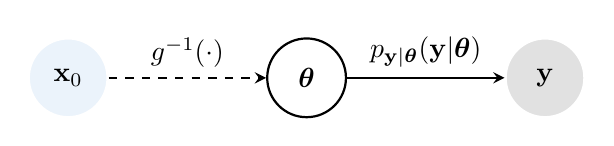
\begin{tikzpicture}[node distance=3cm and 2cm]

% Nodes
\node[latent] (x0) {$\mathbf{x}_{0}$};
\node[observed, right=of x0] (theta) {$\boldsymbol{\theta}$};
\node[data, right=of theta] (y) {$\mathbf{y}$};

% Edges
\draw[dashed_arrow] (x0) -- node[midway, above] {$g^{-1}(\cdot)$} (theta);
\draw[solid_arrow] (theta) -- node[midway, above] {$p_{\mathbf{y}\vert\boldsymbol{\theta}}(\mathbf{y} \vert \boldsymbol{\theta})$} (y);

\end{tikzpicture}


\caption{\textbf{Hierarchical Probabilistic Model.} The dotted arrow represents a deterministic relationship, while the solid arrow indicates a probabilistic relationship.}
\label{fig-graphical-model}
\end{figure}




\subsection{The Evidence Trick}
To approximate the likelihood $p_{\mathbf{y} \vert \mathbf{x}_t}(\mathbf{y} \vert \mathbf{x}_t)$ as defined in~\eqref{eq-likelihood-y-xt}, we propose a simple yet effective approach that we call the \textit{evidence trick}. Given the assumption that the likelihood $p_{\mathbf{y}|\boldsymbol{\theta}}(\mathbf{y}|\boldsymbol{\theta})$ belongs to the exponential family, there always exists a natural conjugate prior distribution $q_{\boldsymbol{\theta}|\boldsymbol{\zeta}}(\boldsymbol{\theta}|\boldsymbol{\zeta})$ with hyperparameters $\boldsymbol{\zeta}$ for which the integral
\begin{equation*}
\int p_{\mathbf{y}|\boldsymbol{\theta}}(\mathbf{y}|\boldsymbol{\theta}) q_{\boldsymbol{\theta}|\boldsymbol{\zeta}}(\boldsymbol{\theta}|\boldsymbol{\zeta}) \mathrm{d}\boldsymbol{\theta} 
\end{equation*}
can be computed in closed-form and corresponds to the \textit{evidence} of $p_{\mathbf{y}|\boldsymbol{\theta}}(\mathbf{y}|\boldsymbol{\theta})$.
As shown in Proposition~\ref{prop:expfam_form_independent_parameters}, the natural conjugate prior distribution also belongs to the exponential family and takes the form:
\begin{equation}
\label{eq-prior-q-theta}
q_{\boldsymbol{\theta}|\boldsymbol{\zeta}}(\boldsymbol{\theta}|\boldsymbol{\zeta}) = h_{\boldsymbol{\theta}}(\boldsymbol{\theta}) \exp \left(\boldsymbol{\zeta}^T \mathbf{T}_{\boldsymbol{\theta}}(\boldsymbol{\theta}) - A_{\boldsymbol{\theta}}(\boldsymbol{\nu},  \boldsymbol{\tau}) \right),
\end{equation}
with hyperparameters $\boldsymbol{\zeta} = \left(\boldsymbol{\nu} ,\boldsymbol{\tau}\right)$, $\boldsymbol{\nu}, \boldsymbol{\tau}  \in \mathbb{R}^d$, base measure $h_{\boldsymbol{\theta}}(\boldsymbol{\theta})$, sufficient statistics $\mathbf{T}_{\boldsymbol{\theta}}(\boldsymbol{\theta}) = (\boldsymbol{\eta}(\boldsymbol{\theta}), -\mathbf{A}_{\boldsymbol{y}}(\boldsymbol{\eta}(\boldsymbol{\theta})))$ and log-partition function $A_{\boldsymbol{\theta}}(\boldsymbol{\nu},  \boldsymbol{\tau})$. The specific form of the natural conjugate prior distribution's base measure and log-partition function is provided in Appendix~\ref{app-table_distributions}.

On this basis, we propose approximating $p_{\boldsymbol{\theta}|\mathbf{x}_t}(\boldsymbol{\theta}|\mathbf{x}_t)$ using the variational distribution $q_{\boldsymbol{\theta}|\boldsymbol{\zeta}(\mathbf{x}_t)}(\boldsymbol{\theta}|\boldsymbol{\zeta}(\mathbf{x}_t))$, as expressed below:
\begin{equation*}
%\label{eq-mean-field-variational-approx}
p_{\boldsymbol{\theta}|\mathbf{x}_t}(\boldsymbol{\theta}|\mathbf{x}_t) \approx q_{\boldsymbol{\theta}|\boldsymbol{\zeta}(\mathbf{x}_t)}(\boldsymbol{\theta}|\boldsymbol{\zeta}(\mathbf{x}_t)),
\end{equation*}
where the dependence of the hyperparameters $\boldsymbol{\zeta}(\mathbf{x}_t)  = \left(\boldsymbol{\nu}(\mathbf{x}_t) ,\boldsymbol{\tau}(\mathbf{x}_t)\right)$ on the input $\mathbf{x}_t$ is explicitly indicated.
This allows us to treat the density $p_{\mathbf{y}|\mathbf{x}_t}(\mathbf{y}|\mathbf{x}_{t})$ as the \textit{evidence} and approximate it with:
\begin{equation}
\label{eq:likelihood_t}
     p_{\mathbf{y}|\mathbf{x}_t}(\mathbf{y}|\mathbf{x}_{t})
     \approx\int p_{\mathbf{y}|\boldsymbol{\theta}}(\mathbf{y}|\boldsymbol{\theta}) q_{\boldsymbol{\theta}|\boldsymbol{\zeta}(\mathbf{x}_t)}(\boldsymbol{\theta}|\boldsymbol{\zeta}(\mathbf{x}_t)) \mathrm{d}\boldsymbol{\theta}.
\end{equation}
As shown in Proposition~\ref{prop:conjugacy}, the integral in \eqref{eq:likelihood_t} has a closed form expression which is given by 
\begin{multline}
\label{eq:likelihood_t-closed-form}
     p_{\mathbf{y}|\mathbf{x}_t}(\mathbf{y}|\mathbf{x}_{t}) \approx \\ h_{\mathbf{y}}(\mathbf{y}) \frac{\exp\left(-A_{\boldsymbol{\theta}}(\boldsymbol{\nu}(\mathbf{x}_t), \boldsymbol{\tau}(\mathbf{x}_t))\right)}{\exp\left(-A_{\boldsymbol{\theta}}(\mathbf{T}_{\mathbf{y}}(\mathbf{y}) + \boldsymbol{\nu}(\mathbf{x}_t), \boldsymbol{\tau}(\mathbf{x}_t) + N \mathbf{1}_d)\right)}.
\end{multline}

\subsection{Approximate Inference of  
$p_{\protect\boldsymbol{\theta}|\mathbf{x}_t}(\protect\boldsymbol{\theta}|\mathbf{x}_t)$}

In this section, we outline the process of finding the optimal approximation to $p_{\boldsymbol{\theta}|\mathbf{x}_t}(\boldsymbol{\theta}|\mathbf{x}_{t})$ by minimizing the KL divergence relative to $q_{\boldsymbol{\theta}\vert \boldsymbol{\zeta}(\mathbf{x}_t)}(\boldsymbol{\theta}\vert \boldsymbol{\zeta}(\mathbf{x}_t))$. For the next result, it is convenient to denote the log-partition function of the conjugate prior defined in~\eqref{eq-prior-q-theta} with $A_{\boldsymbol{\theta}}(\boldsymbol{\zeta}(\mathbf{x}_t)) := A_{\boldsymbol{\theta}}(\boldsymbol{\nu}(\mathbf{x}_t), \boldsymbol{\tau}(\mathbf{x}_t))$.
\begin{lemma}[KL Divergence of $p_{\boldsymbol{\theta}\vert \mathbf{x}_t}$ from $q_{\boldsymbol{\theta}\vert \boldsymbol{\zeta}(\mathbf{x}_t)}$]
\label{lemma-KL-divergence}
Let~$\boldsymbol{\theta} = g^{-1}(\mathbf{x}_0)$.
Furthermore, let
$q_{\boldsymbol{\theta}\vert \boldsymbol{\zeta}(\mathbf{x}_t)}(\boldsymbol{\theta}\vert \boldsymbol{\zeta}(\mathbf{x}_t))$ be defined as in~\eqref{eq-prior-q-theta} and be part of the exponential family with
hyperparameters $\boldsymbol{\zeta}(\mathbf{x}_t)$, base measure $h_{\boldsymbol{\theta}}(\boldsymbol{\theta})$, sufficient statistics $\mathbf{T}_{\boldsymbol{\theta}}(\boldsymbol{\theta})$ and
log-partition function $A_{\boldsymbol{\theta}}(\boldsymbol{\zeta}(\mathbf{x}_t))$.  
The KL divergence of $p_{\boldsymbol{\theta}\vert \mathbf{x}_t}$ from $q_{\boldsymbol{\theta}\vert \boldsymbol{\zeta}(\mathbf{x}_t)}$ is given by
\begin{equation}
\label{eq-kl-divergence-exp}
    D_{\text{KL}}(p_{\boldsymbol{\theta}\vert \mathbf{x}_t} \vert\vert q_{\boldsymbol{\theta}\vert \boldsymbol{\zeta}(\mathbf{x}_t)}) =  C(\mathbf{x}_t)  +\mathcal{L}_{\text{AVI}}(\boldsymbol{\zeta}, \mathbf{x}_t)
\end{equation}
where 
\begin{multline*}
\mathcal{L}_{\text{AVI}}\left(\boldsymbol{\zeta},\mathbf{x}_t\right) =\\  A_{\boldsymbol{\theta}}(\boldsymbol{\zeta}(\mathbf{x}_t)) -\boldsymbol{\zeta}(\mathbf{x}_t)^{\top}\mathbb{E}_{p_{\tilde{\mathbf{x}}_{0}\vert\mathbf{x}_t}}[\mathbf{T}_{\boldsymbol{\theta}}(g^{-1}(\tilde{\mathbf{x}}_{0}))]
\end{multline*}
and for a function $C(\mathbf{x}_t)$ that does not depend on $\boldsymbol{\zeta}$.
\end{lemma}
The proof of Lemma \ref{lemma-KL-divergence} is postponed to Appendix \ref{sec:proof_lemma-KL-divergence}.
We define $\boldsymbol{\zeta}^{\star}(\mathbf{x}_t)$ as the set of hyperparameters that minimizes the KL divergence in~\eqref{eq-kl-divergence-exp} for a given input $\mathbf{x}_t$. Furthermore, let  $\boldsymbol{\zeta}^{\star}(\cdot)$ denote the function that minimizes the expected KL divergence, as specified by the objective
\begin{equation}
\label{eq-kl-expectation}
\mathcal{J}_{\text{AVI}}(\boldsymbol{\zeta}) = \mathbb{E}_{t\sim U(\epsilon, 1), \mathbf{x}_t \sim p_{\mathbf{x}_t}}\Big[ \mathcal{L}_{\text{AVI}}(\boldsymbol{\zeta},\mathbf{x}_t,t)\Big].
\end{equation}
where the function $C(\mathbf{x}_t)$ in~\eqref{eq-kl-divergence-exp} has been excluded from the optimization, as it does not depend on $\boldsymbol{\zeta}$. 
A significant challenge in optimizing~\eqref{eq-kl-expectation} arises from the term $\mathbb{E}_{p_{\tilde{\mathbf{x}}_{0}|\mathbf{x}_t}}[\mathbf{T}_{\boldsymbol{\theta}}(g^{-1}(\tilde{\mathbf{x}}_{0}))]$. This term requires computing expectations under the reverse process distribution $p_{\tilde{\mathbf{x}}_{0}|\mathbf{x}_t}$, which is generally intractable. To address this issue, our next result demonstrates that the objective in~\eqref{eq-kl-expectation} can be reformulated in a way that entirely avoids this explicit evaluation.
\begin{theorem}
\label{prop-new-objective}
Let $p_{\boldsymbol{\theta}}(\boldsymbol{\theta})$ be the marginal distribution of $\boldsymbol{\theta}$.  Moreover, assume that $\boldsymbol{\zeta}(\cdot)$ is a Lipschitz continuous function and that the following conditions hold:
\begin{equation*}
%\label{eq-condition-theorem}
\begin{aligned}
\mathbb{E}_{\boldsymbol{\theta}\sim  p_{\boldsymbol{\theta}}}[\norm{\mathbf{T}_{\boldsymbol{\theta}}(\boldsymbol{\theta}) }] &< \infty,\\
\mathbb{E}_{\boldsymbol{\theta}\sim  p_{\boldsymbol{\theta}}}[\norm{g(\boldsymbol{\theta})}\norm{\mathbf{T}_{\boldsymbol{\theta}}(\boldsymbol{\theta}) }] &< \infty 
\end{aligned}
\end{equation*}
Then, the objective in~\eqref{eq-kl-expectation} can be equivalently expressed as:
% \begin{multline}
%  \boldsymbol{\zeta}^{\star}(\cdot) = \argminA_{\boldsymbol{\zeta}(\cdot)} \mathbb{E}_{t\sim U(\epsilon, 1), \mathbf{x}_0\sim  p_{\mathbf{x}_0}, \mathbf{x}_t \sim p_{\mathbf{x}_t|\mathbf{x}_0}}\Big[ A_{\boldsymbol{\theta}}(\boldsymbol{\zeta}(\mathbf{x}_t)) \\ - \boldsymbol{\zeta}(\mathbf{x}_t)^{\top}\mathbf{T}_{\boldsymbol{\theta}}(g^{-1}(\mathbf{x}_{0}))\Big].
% \end{multline}
\begin{multline}
\label{eq-amortized-objective}
\mathcal{J}_{\text{AVI}}(\boldsymbol{\zeta}) = \\  \mathbb{E}_{t\sim U(\epsilon, 1), \mathbf{x}_0\sim  p_{\mathbf{x}_0}, \mathbf{x}_t \sim p_{\mathbf{x}_t|\mathbf{x}_0}}\Big[ \tilde{\mathcal{L}}_{\text{AVI}}(\boldsymbol{\zeta}, \mathbf{x}_0,\mathbf{x}_t)\Big]
\end{multline}
where
\begin{multline*}
\tilde{\mathcal{L}}_{\text{AVI}}(\boldsymbol{\zeta}, \mathbf{x}_0,\mathbf{x}_t) =  A_{\boldsymbol{\theta}}(\boldsymbol{\zeta}(\mathbf{x}_t))  - \boldsymbol{\zeta}(\mathbf{x}_t)^{\top}\mathbf{T}_{\boldsymbol{\theta}}(g^{-1}(\mathbf{x}_{0})).
\end{multline*}
\end{theorem}
The proof of Theorem~\ref{prop-new-objective} is deferred to Appendix~\ref{proof-prop-new-objective}. 
To approximate $\boldsymbol{\zeta}^{\star}(\cdot)$, we adopt the framework of \textit{amortized variational inference} (AVI).
We use a neural network, denoted by $\boldsymbol{\zeta}_{\boldsymbol{\rho}}(\mathbf{x}_t, t)$ where $\boldsymbol{\rho}$ represents the trainable parameters of the network. We train the neural network such that the parameters $\boldsymbol{\rho}^{*}$ are a minimizer of the following amortized objective:
\begin{multline*}
%\label{eq-amortized-objective}
\mathcal{J}_{\text{AVI}}(\boldsymbol{\rho}) = \\ \mathbb{E}_{t\sim U(\epsilon, 1), \mathbf{x}_0\sim  p_{\mathbf{x}_0},\mathbf{x}_t \sim p_{\mathbf{x}_t|\mathbf{x}_0}}\Big[ \tilde{\mathcal{L}}_{\text{AVI}}(\boldsymbol{\rho},\mathbf{x}_0,\mathbf{x}_t, t)\Big]
\end{multline*}
where
\begin{multline*}
\tilde{\mathcal{L}}_{\text{AVI}}(\boldsymbol{\rho},\mathbf{x}_0,\mathbf{x}_t, t) =  \\  A_{\boldsymbol{\theta}}(\boldsymbol{\zeta}_{\boldsymbol{\rho}}(\mathbf{x}_t, t))  -\boldsymbol{\zeta}_{\boldsymbol{\rho}}(\mathbf{x}_t, t)^{\top}\mathbf{T}_{\boldsymbol{\theta}}(g^{-1}(\mathbf{x}_{0})).
\end{multline*}
\begin{remark}[Inference Network]
The function $\boldsymbol{\zeta}_{\boldsymbol{\rho}}(\mathbf{x}_t,t)$ serves as an \textit{inference network} that infers a posterior distribution over the original (denoised) parameter vector $\boldsymbol{\theta}$, conditioned on its progressively noised counterpart 
$\mathbf{x}_t$ at diffusion time step $t$. Implemented via a neural network, $\boldsymbol{\zeta}_{\boldsymbol{\rho}}$  maps the noisy input $\mathbf{x}_t$ and timestep $t$ to the parameters of this posterior distribution, effectively approximating the inverse of the forward noising process.
\end{remark}




%% TODO UPDATE THIS REMARK
% \begin{remark}[Conditions for Gaussian prior distribution]
% Assuming $p_{\boldsymbol{\theta}}(\boldsymbol{\theta})$ is a multivariate Gaussian distribution and $g(
% \boldsymbol{\theta}) = \boldsymbol{\theta}$, the conditions in~\eqref{eq-condition-theorem} reduce to 
% \begin{equation}
% \begin{aligned}
% \mathbb{E}_{p_{\boldsymbol{\theta}}}[\vert\boldsymbol{\theta} \vert ] &< \infty \\
% \mathbb{E}_{p_{\boldsymbol{\theta}}}[||\boldsymbol{\theta}||^{2} ] &< \infty,
% \end{aligned}
% \end{equation}
% which are trivially satisfied for any multivariate Gaussian distribution.
% \end{remark}

\subsection{Computing the Score of $p_{\mathbf{y}|\mathbf{x}_t}(\mathbf{y}|\mathbf{x}_{t})$}
To sample from the posterior using diffusion models, it is necessary to approximate the likelihood score function, $\nabla_{\mathbf{x}_t} \log p_{\mathbf{y} \vert \mathbf{x}_t}(\mathbf{y} \vert \mathbf{x}_t)$, as defined in~\eqref{eq:score_posterior}. 
From~\eqref{eq:likelihood_t-closed-form}, the log-density $\log p_{\mathbf{y}|\mathbf{x}_t}(\mathbf{y}|\mathbf{x}_t)$ can be directly approximated with
\begin{multline*}
    \log p_{\mathbf{y}|\mathbf{x}_t}(\mathbf{y}|\mathbf{x}_{t})
     \approx \log h_{\mathbf{y}}(\mathbf{y}) - A_{\boldsymbol{\theta}}(\boldsymbol{\nu}(\mathbf{x}_t), \boldsymbol{\tau}(\mathbf{x}_t)) \\+ A_{\boldsymbol{\theta}}(\mathbf{T}_{\mathbf{y}}(\mathbf{y}) + \boldsymbol{\nu}(\mathbf{x}_t), \boldsymbol{\tau}(\mathbf{x}_t) + N \mathbf{1}_d).
\end{multline*}
The gradient of the log-density,~$\nabla_{\mathbf{x}_t} \log  p_{\mathbf{y}|\mathbf{x}_t}(\mathbf{y}|\mathbf{x}_{t})$ with respect to $\mathbf{x}_t$ can be efficiently computed using automatic differentiation.  




\section{Experiments} \label{sec:experiment}
The technical details of each experiment discussed in this section can be found in Appendix~\ref{app-experiment-set-up}. The first experiment demonstrates the effectiveness of our method in approximating a posterior distribution that closely aligns with the ground truth obtained via MCMC, using a hierarchical model where the prior can be evaluated. The final two experiments address scenarios where an empirical prior is used, making MCMC infeasible.

\begin{figure*}[t!]
\centering
\includegraphics[width=\textwidth]{plots/main_poisson_images.pdf}
\caption{\textbf{Score-Based Cox Process Results.} \textbf{(a)} (Left) True Cox Process intensity from the ImageNet validation set, transformed using an exponential link function. (Right) Median of the estimated Cox Process intensity posterior distribution using the Score-Based Cox Process method. \textbf{(b)} (Left) True Cox Process Intensity from Sentinel-2 Satellite Imagery of Manhattan, New York City (Right) Median of the estimated Cox Process intensity posterior distribution using the Score-Based Cox Process method.}
\label{fig:imagenet-cox-process}
\end{figure*} 

\subsection{One-dimensional Benchmark Analysis}
\label{sec-1d-synthetic-data}
We developed a simple one-dimensional experiment to illustrate the effectiveness of our method in approximating a posterior distribution that closely aligns with the ground truth obtained through MCMC.
This experiment also serves as a basis for comparing our posterior approximation with that generated by the DPS method. 
We consider the following hierarchical generative model:
\begin{equation*}
y_{i,j} \sim \text{Poisson}(\theta_j), \quad \boldsymbol{\theta} = \exp(\mathbf{x}_0), \quad \mathbf{x}_0 \sim \mathcal{GP}(0, \mathbf{K})
\end{equation*}
for $i = 1, \ldots, N$ and $j = 1, \dots d$, where $d = 30$ and $\mathbf{K}$ is the Gaussian Process (GP) covariance matrix defined by a radial basis function (RBF) kernel with variance 1 and length-scale 0.1. 
Using this model, we generated synthetic observations. We aim to solve the inverse problem of recovering the unknown Poisson intensity $\boldsymbol{\theta}$ from the generated synthetic observations. We used as a prior the true latent variable Gaussian Process distribution. 

We compared the posterior distribution of $\boldsymbol{\theta}$ estimated by our method against the ground-truth MCMC posterior as well as the DPS posterior approximation. 
The results of this comparison are provided in Appendix~\ref{app-results-synthetic-1d}.
Our approach demonstrates significantly better alignment with the ground-truth MCMC posterior. In contrast, DPS fails to accurately capture both the credible intervals and the point estimates.
To further assess robustness, we repeated this experiment using other distributions within the exponential family, for which DPS could not be used. Our method consistently aligned with the ground-truth MCMC posterior distribution. 
% The right panel contrasts the predictive distributions: our method better recovers the data-generating process, whereas DPS shows systematic bias in regions of low observation density.
% To assess robustness, we repeated the experiment with Pareto and Exponential likelihoods (Appendix~\ref{app-results-synthetic-1d}). Our method maintains consistent performance across all likelihood families.


\subsection{Score-Based Cox Process}
\label{sec-experiment-cox-process}
A Cox process, also called a doubly stochastic Poisson process, is a point process that generalizes the Poisson process by allowing its intensity function to be governed by a stochastic process, varying across the underlying mathematical space. The space over which the intensity function is defined is discretized to be a $256 \times 256$ grid. Each grid cell's observation is a Poisson random variable, parameterized by the corresponding intensity value.

To generate synthetic Cox Process observations, we explored multiple intensities including samples from the ImageNet validation dataset, a satellite image, and a map of buildings' heights in London. For each choice of intensity, we drew $N = 50$ event samples according to a Cox Process and allocated 80\% of the grid cells to the training set and the remaining 20\% to the test set.

To address the inverse problem, we employed the ImageNet prior. This prior assumes that $\mathbf{x}_0$ are samples from the ImageNet train dataset. We use the exponential inverse link function. The hierarchical generative model was:
\begin{equation*}
y_{i,j} \sim \text{Poisson}(\theta_j), \quad
\boldsymbol{\theta} = \exp(\mathbf{x}_0), \quad
\mathbf{x}_0 \sim \text{ImageNet}
\end{equation*}
for $i = 1, \ldots, N$, $j = 1, \ldots d$, and where $d = 256\times 256$. We refer to this method as the \textit{``Score-Based Cox Process"}. It should be noted that MCMC inference cannot be used due to the intractability of the prior density.
Figure~\ref{fig:imagenet-cox-process} shows the results of the \textit{``Score-Based Cox Process"} on recovering the true intensity surface. Further experimental results given different values of $N$ and different intensities are provided in Appendix~\ref{app-further-experiment-cox-process}. 



\subsection{Prevalence of Malaria Prevalence in Sub-Saharan Africa}
\label{sec-experiment-malaria}
The \emph{Plasmodium falciparum} parasite rate (PfPR) quantifies the proportion of individuals who have the malaria parasite. The data used to estimate the PfPR consist of the number of positive cases in location $j$, denoted as $y_j$ (detected using rapid diagnostic tests or PCR), out of the total number of individuals examined in the same location, $n_j$. Spatio-temporal mapping of PfPR is typically conducted using GPs~\cite{Bhatt2015-uk}. However, the growing volume of data has rendered full-rank Bayesian inference with GPs computationally impractical. Furthermore, the simple covariance functions commonly used in GPs may be inadequate, necessitating increasingly complex models to accurately predict PfPR across spatial and temporal dimensions \cite{Bhatt2017-tk}. 
Here, we reanalyzed a real-world dataset on PfPR from the Malaria Atlas Project, previously used to monitor malaria trends in Sub-Saharan Africa~\citep{Bhatt2015-uk,Pfeffer2018-cm, Weiss2019-au} --- the continent bearing the highest burden of the disease. 
We ignored temporal aspects, and only aimed to interpolate spatial data across all of Sub-Saharan Africa. We used a grid resolution of $256 \times 256$, equivalent to a $\sim 111 \text{ km}^2$ resolution, and aggregated positive cases and individuals examined to this resolution. Out of the grid, $7,048$ ($10.75$\%) entries had non-missing observations, which were then split into training and test sets in an 80/20 ratio. The hierarchical generative model was:
\begin{equation*}
y_{j} \sim \text{Binomial}(n_j,\theta_j), \; \boldsymbol{\theta} = \sigma(s\,\mathbf{x}_0), \;
\mathbf{x}_0 \sim \text{ImageNet}
\end{equation*}
for $j = 1, \ldots d$, $s = 5$ and where $d = 256\times 256$, and where $\sigma(\cdot)$ is the sigmoid (inverse logit) function.
Figure~\ref{fig:malaria-results} presents the PfPR posterior median and credible interval estimated using our approach. A benchmark analysis comparing our method to the Gaussian Markov Random Field (GMRF) --- considered the state-of-the-art for disease mapping~\citep{Rue2009-ty, Lindgren2011-fv, Heaton2017-vl} --- is provided in Appendix~\ref{app-further-experiment-malaria}. Our results show that our approach performs competitively with the GMRF model.

\begin{figure*}[ht!]
\centering
\includegraphics[width=\textwidth]{plots/malaria_plot_main.pdf}
\caption{\textbf{Prevalence of Malaria in Sub-Saharan Africa Results.} \textbf{(a)} Empirical PfPR. \textbf{(b)} Median of the estimated PfPR posterior distribution. \textbf{(c)} $25$\% quantile of the estimated PfPR posterior distribution. \textbf{(d)} $75$\% quantile of the estimated PfPR posterior distribution. 
The inset plots highlight Nigeria, one of the countries with the highest malaria burden worldwide.
The empty entries either correspond to locations outside Sub-Saharan Africa or the stable spatial limits of \emph{P. falciparum} transmission~\cite{Bhatt2015-uk} }
\label{fig:malaria-results}
\end{figure*}





\section{Related Work}\label{sec:related_work}
Since our work focuses on addressing inverse problems with non-Gaussian observations, we review several approaches that have also attempted to solve this problem.

\paragraph{Markov Chain Monte Carlo.} MCMC is the most commonly used posterior sampling method for performing Bayesian inference on inverse problems.  A key characteristic of MCMC methods is the need to evaluate the prior to compute the acceptance rate for candidate samples generated by the proposal distribution. This requirement presents a significant limitation compared to diffusion-based approaches, which only require the ability to sample from the prior distribution. Therefore, diffusion-based methods accommodate a much broader range of prior distributions.


\paragraph{Gaussian Process and Gaussian Markov Random Field.} GPs are widely used for modeling latent functions in tasks where capturing uncertainty is crucial but are computationally expensive due to the worst-case cubic complexity of inverting large covariance matrices \citep{Rasmussen_GP, Adams2009}. For non-Gaussian observations, Bayesian inference can only be performed via MCMC sampling, which suffers from autocorrelation and slow mixing, making it impractical for large-scale experiments. Given our dataset size and parameter dimensionality, MCMC-based GP inference was infeasible.

As an alternative to MCMC, the most popular approximate method is the integrated nested Laplace approximation (INLA) \cite{Rue2005}, combined with GMRFs. INLA enables sparse computations and avoids MCMC’s mixing issues through an optimization-based approach. However, INLA has limitations: it restricts covariance functions to stationary ones, struggles with high spectral frequencies \cite{Stein2014-hc}, lacks posterior accuracy guarantees, and makes obtaining posterior samples challenging.


% Finally, conditional simulation and sampling can also be challenging~\cite{Rasmussen_GP}.




\paragraph{Diffusion Posterior Sampling.} Among existing diffusion models-based methodologies, we mention DPS, the work of~\citet{chung2023}, who proposed to approximate $p_{\mathbf{x}_{0}\vert\mathbf{x}_t}(\mathbf{x}_0 \vert \mathbf{x}_t)$ as a Dirac delta distribution centered at the posterior mean $\mathbb{E}_{\mathbf{x}_{0}\sim p_{\mathbf{x}_{0}\vert\mathbf{x}_t}}[\mathbf{x}_0]$.
The latter is determined using Tweedie’s formula. Although their method was originally designed for linear inverse problems with Gaussian likelihoods, the authors also extended it to address inverse problems involving Poisson-distributed observations. 
This approach relies on the assumption that Gaussian distributions can effectively approximate Poisson-distributed data when the rate is sufficiently high. However, as noted in \citep[Appendix C.4]{chung2023} and illustrated in the experiment presented in Section~\ref{sec-1d-synthetic-data}, the method faces numerical instabilities and produces poor approximations when the observations come from a low-rate Poisson distribution. Furthermore, the method depends on Tweedie’s formula, which is known to exhibit high variance at high noise levels during the reverse diffusion process (see Section 1.2 of~\citet{target_score_matching}).


\paragraph{Simulation-Based Inference (SBI).} 
SBI avoids the need for a tractable likelihood by relying on simulated observations. Diffusion models enable SBI by approximating the likelihood score function through a Conditional Denoising Estimator (CDE) in the form of a neural network. The CDE directly estimates the likelihood score function by conditioning on three inputs: the observations $\mathbf{y}$, the noise-corrupted latent variable $\mathbf{x}_t$ and the diffusion timestep $t$~\citep{batzolis2021,simons2023}.

Existing approaches face three critical limitations. First, using observations 
$\mathbf{y}$ as network input requires retraining for each new dataset, incurring high computational costs.
Second, in a multiple samples regime ($N>1$), the likelihood score function depends on both the prior and the likelihood score networks~\citep{geffner23a}, causing errors from the prior network to propagate into the likelihood approximation. Third, these methods struggle to accommodate heterogeneous missing data patterns across observations. This limitation stems from their reliance on a fixed input structure for $\mathbf{y}$: missing observations can only be processed if they conform to the network's predefined input format, restricting their applicability to real-world datasets with variable or unanticipated missingness. In contrast, our approach trains a single network given a choice of likelihood, decoupling it from the specific missing-data pattern and the observations themselves. 
%This ensures robustness to heterogeneous missingness and eliminates computational overhead from repeated training, achieving both efficiency and real-world applicability.









\section{Conclusion} \label{sec:conclusion}
In this work, we introduced a novel approach for solving inverse problems using diffusion models when observations follow distributions from the exponential family. 
Our posterior approximation closely aligns with MCMC methods while scaling to larger observational datasets and accommodating empirical priors. We demonstrate strong performance in image denoising under Poisson noise and further highlight the method’s effectiveness in real-world problems. Notably, our results suggest that an ImageNet prior can be a powerful tool for spatial statistics, enabling the recovery of latent patterns that extend beyond those present in ImageNet itself.

\section*{Impact Statement}
\section*{Impact Statement}
We introduce \sys, an AI agent framework designed to ensure methodical control, execution reliability, and structured knowledge management throughout the experimentation lifecycle.
We introduce a novel experimentation benchmark, spanning four key domains in computer science, to evaluate the reliability and effectiveness of AI agents in conducting scientific research. Our empirical results demonstrate that \sys achieves higher conclusion accuracy and execution reliability, significantly outperforming state-of-the-art AI agents.


\sys has broad implications across multiple scientific disciplines, including machine learning, cloud computing, and database systems, where rigorous experimentation is essential. Beyond computer science, our framework has the potential to accelerate research in materials science, physics, and biomedical research, where complex experimental setups and iterative hypothesis testing are critical for discovery. By automating experimental workflows with built-in validation, \sys can enhance research productivity, reduce human error, and facilitate large-scale scientific exploration.

Ensuring transparency, fairness, and reproducibility in AI-driven scientific research is paramount. \sys explicitly enforces structured documentation and interpretability, making experimental processes auditable and traceable. However, over-reliance on AI for scientific discovery raises concerns regarding bias in automated decision-making and the need for human oversight. We advocate for hybrid human-AI collaboration, where AI assists researchers rather than replacing critical scientific judgment.

\sys lays the foundation for trustworthy AI-driven scientific experimentation, opening avenues for self-improving agents that refine methodologies through continual learning. Future research could explore domain-specific adaptations, enabling AI to automate rigorous experimentation in disciplines such as drug discovery, materials engineering, and high-energy physics. By bridging AI and the scientific method, \sys has the potential to shape the next generation of AI-powered research methodologies, driving scientific discovery at an unprecedented scale.










\bibliography{ref}
\bibliographystyle{style/icml2025}

\appendix
\onecolumn
\subsection{Lloyd-Max Algorithm}
\label{subsec:Lloyd-Max}
For a given quantization bitwidth $B$ and an operand $\bm{X}$, the Lloyd-Max algorithm finds $2^B$ quantization levels $\{\hat{x}_i\}_{i=1}^{2^B}$ such that quantizing $\bm{X}$ by rounding each scalar in $\bm{X}$ to the nearest quantization level minimizes the quantization MSE. 

The algorithm starts with an initial guess of quantization levels and then iteratively computes quantization thresholds $\{\tau_i\}_{i=1}^{2^B-1}$ and updates quantization levels $\{\hat{x}_i\}_{i=1}^{2^B}$. Specifically, at iteration $n$, thresholds are set to the midpoints of the previous iteration's levels:
\begin{align*}
    \tau_i^{(n)}=\frac{\hat{x}_i^{(n-1)}+\hat{x}_{i+1}^{(n-1)}}2 \text{ for } i=1\ldots 2^B-1
\end{align*}
Subsequently, the quantization levels are re-computed as conditional means of the data regions defined by the new thresholds:
\begin{align*}
    \hat{x}_i^{(n)}=\mathbb{E}\left[ \bm{X} \big| \bm{X}\in [\tau_{i-1}^{(n)},\tau_i^{(n)}] \right] \text{ for } i=1\ldots 2^B
\end{align*}
where to satisfy boundary conditions we have $\tau_0=-\infty$ and $\tau_{2^B}=\infty$. The algorithm iterates the above steps until convergence.

Figure \ref{fig:lm_quant} compares the quantization levels of a $7$-bit floating point (E3M3) quantizer (left) to a $7$-bit Lloyd-Max quantizer (right) when quantizing a layer of weights from the GPT3-126M model at a per-tensor granularity. As shown, the Lloyd-Max quantizer achieves substantially lower quantization MSE. Further, Table \ref{tab:FP7_vs_LM7} shows the superior perplexity achieved by Lloyd-Max quantizers for bitwidths of $7$, $6$ and $5$. The difference between the quantizers is clear at 5 bits, where per-tensor FP quantization incurs a drastic and unacceptable increase in perplexity, while Lloyd-Max quantization incurs a much smaller increase. Nevertheless, we note that even the optimal Lloyd-Max quantizer incurs a notable ($\sim 1.5$) increase in perplexity due to the coarse granularity of quantization. 

\begin{figure}[h]
  \centering
  \includegraphics[width=0.7\linewidth]{sections/figures/LM7_FP7.pdf}
  \caption{\small Quantization levels and the corresponding quantization MSE of Floating Point (left) vs Lloyd-Max (right) Quantizers for a layer of weights in the GPT3-126M model.}
  \label{fig:lm_quant}
\end{figure}

\begin{table}[h]\scriptsize
\begin{center}
\caption{\label{tab:FP7_vs_LM7} \small Comparing perplexity (lower is better) achieved by floating point quantizers and Lloyd-Max quantizers on a GPT3-126M model for the Wikitext-103 dataset.}
\begin{tabular}{c|cc|c}
\hline
 \multirow{2}{*}{\textbf{Bitwidth}} & \multicolumn{2}{|c|}{\textbf{Floating-Point Quantizer}} & \textbf{Lloyd-Max Quantizer} \\
 & Best Format & Wikitext-103 Perplexity & Wikitext-103 Perplexity \\
\hline
7 & E3M3 & 18.32 & 18.27 \\
6 & E3M2 & 19.07 & 18.51 \\
5 & E4M0 & 43.89 & 19.71 \\
\hline
\end{tabular}
\end{center}
\end{table}

\subsection{Proof of Local Optimality of LO-BCQ}
\label{subsec:lobcq_opt_proof}
For a given block $\bm{b}_j$, the quantization MSE during LO-BCQ can be empirically evaluated as $\frac{1}{L_b}\lVert \bm{b}_j- \bm{\hat{b}}_j\rVert^2_2$ where $\bm{\hat{b}}_j$ is computed from equation (\ref{eq:clustered_quantization_definition}) as $C_{f(\bm{b}_j)}(\bm{b}_j)$. Further, for a given block cluster $\mathcal{B}_i$, we compute the quantization MSE as $\frac{1}{|\mathcal{B}_{i}|}\sum_{\bm{b} \in \mathcal{B}_{i}} \frac{1}{L_b}\lVert \bm{b}- C_i^{(n)}(\bm{b})\rVert^2_2$. Therefore, at the end of iteration $n$, we evaluate the overall quantization MSE $J^{(n)}$ for a given operand $\bm{X}$ composed of $N_c$ block clusters as:
\begin{align*}
    \label{eq:mse_iter_n}
    J^{(n)} = \frac{1}{N_c} \sum_{i=1}^{N_c} \frac{1}{|\mathcal{B}_{i}^{(n)}|}\sum_{\bm{v} \in \mathcal{B}_{i}^{(n)}} \frac{1}{L_b}\lVert \bm{b}- B_i^{(n)}(\bm{b})\rVert^2_2
\end{align*}

At the end of iteration $n$, the codebooks are updated from $\mathcal{C}^{(n-1)}$ to $\mathcal{C}^{(n)}$. However, the mapping of a given vector $\bm{b}_j$ to quantizers $\mathcal{C}^{(n)}$ remains as  $f^{(n)}(\bm{b}_j)$. At the next iteration, during the vector clustering step, $f^{(n+1)}(\bm{b}_j)$ finds new mapping of $\bm{b}_j$ to updated codebooks $\mathcal{C}^{(n)}$ such that the quantization MSE over the candidate codebooks is minimized. Therefore, we obtain the following result for $\bm{b}_j$:
\begin{align*}
\frac{1}{L_b}\lVert \bm{b}_j - C_{f^{(n+1)}(\bm{b}_j)}^{(n)}(\bm{b}_j)\rVert^2_2 \le \frac{1}{L_b}\lVert \bm{b}_j - C_{f^{(n)}(\bm{b}_j)}^{(n)}(\bm{b}_j)\rVert^2_2
\end{align*}

That is, quantizing $\bm{b}_j$ at the end of the block clustering step of iteration $n+1$ results in lower quantization MSE compared to quantizing at the end of iteration $n$. Since this is true for all $\bm{b} \in \bm{X}$, we assert the following:
\begin{equation}
\begin{split}
\label{eq:mse_ineq_1}
    \tilde{J}^{(n+1)} &= \frac{1}{N_c} \sum_{i=1}^{N_c} \frac{1}{|\mathcal{B}_{i}^{(n+1)}|}\sum_{\bm{b} \in \mathcal{B}_{i}^{(n+1)}} \frac{1}{L_b}\lVert \bm{b} - C_i^{(n)}(b)\rVert^2_2 \le J^{(n)}
\end{split}
\end{equation}
where $\tilde{J}^{(n+1)}$ is the the quantization MSE after the vector clustering step at iteration $n+1$.

Next, during the codebook update step (\ref{eq:quantizers_update}) at iteration $n+1$, the per-cluster codebooks $\mathcal{C}^{(n)}$ are updated to $\mathcal{C}^{(n+1)}$ by invoking the Lloyd-Max algorithm \citep{Lloyd}. We know that for any given value distribution, the Lloyd-Max algorithm minimizes the quantization MSE. Therefore, for a given vector cluster $\mathcal{B}_i$ we obtain the following result:

\begin{equation}
    \frac{1}{|\mathcal{B}_{i}^{(n+1)}|}\sum_{\bm{b} \in \mathcal{B}_{i}^{(n+1)}} \frac{1}{L_b}\lVert \bm{b}- C_i^{(n+1)}(\bm{b})\rVert^2_2 \le \frac{1}{|\mathcal{B}_{i}^{(n+1)}|}\sum_{\bm{b} \in \mathcal{B}_{i}^{(n+1)}} \frac{1}{L_b}\lVert \bm{b}- C_i^{(n)}(\bm{b})\rVert^2_2
\end{equation}

The above equation states that quantizing the given block cluster $\mathcal{B}_i$ after updating the associated codebook from $C_i^{(n)}$ to $C_i^{(n+1)}$ results in lower quantization MSE. Since this is true for all the block clusters, we derive the following result: 
\begin{equation}
\begin{split}
\label{eq:mse_ineq_2}
     J^{(n+1)} &= \frac{1}{N_c} \sum_{i=1}^{N_c} \frac{1}{|\mathcal{B}_{i}^{(n+1)}|}\sum_{\bm{b} \in \mathcal{B}_{i}^{(n+1)}} \frac{1}{L_b}\lVert \bm{b}- C_i^{(n+1)}(\bm{b})\rVert^2_2  \le \tilde{J}^{(n+1)}   
\end{split}
\end{equation}

Following (\ref{eq:mse_ineq_1}) and (\ref{eq:mse_ineq_2}), we find that the quantization MSE is non-increasing for each iteration, that is, $J^{(1)} \ge J^{(2)} \ge J^{(3)} \ge \ldots \ge J^{(M)}$ where $M$ is the maximum number of iterations. 
%Therefore, we can say that if the algorithm converges, then it must be that it has converged to a local minimum. 
\hfill $\blacksquare$


\begin{figure}
    \begin{center}
    \includegraphics[width=0.5\textwidth]{sections//figures/mse_vs_iter.pdf}
    \end{center}
    \caption{\small NMSE vs iterations during LO-BCQ compared to other block quantization proposals}
    \label{fig:nmse_vs_iter}
\end{figure}

Figure \ref{fig:nmse_vs_iter} shows the empirical convergence of LO-BCQ across several block lengths and number of codebooks. Also, the MSE achieved by LO-BCQ is compared to baselines such as MXFP and VSQ. As shown, LO-BCQ converges to a lower MSE than the baselines. Further, we achieve better convergence for larger number of codebooks ($N_c$) and for a smaller block length ($L_b$), both of which increase the bitwidth of BCQ (see Eq \ref{eq:bitwidth_bcq}).


\subsection{Additional Accuracy Results}
%Table \ref{tab:lobcq_config} lists the various LOBCQ configurations and their corresponding bitwidths.
\begin{table}
\setlength{\tabcolsep}{4.75pt}
\begin{center}
\caption{\label{tab:lobcq_config} Various LO-BCQ configurations and their bitwidths.}
\begin{tabular}{|c||c|c|c|c||c|c||c|} 
\hline
 & \multicolumn{4}{|c||}{$L_b=8$} & \multicolumn{2}{|c||}{$L_b=4$} & $L_b=2$ \\
 \hline
 \backslashbox{$L_A$\kern-1em}{\kern-1em$N_c$} & 2 & 4 & 8 & 16 & 2 & 4 & 2 \\
 \hline
 64 & 4.25 & 4.375 & 4.5 & 4.625 & 4.375 & 4.625 & 4.625\\
 \hline
 32 & 4.375 & 4.5 & 4.625& 4.75 & 4.5 & 4.75 & 4.75 \\
 \hline
 16 & 4.625 & 4.75& 4.875 & 5 & 4.75 & 5 & 5 \\
 \hline
\end{tabular}
\end{center}
\end{table}

%\subsection{Perplexity achieved by various LO-BCQ configurations on Wikitext-103 dataset}

\begin{table} \centering
\begin{tabular}{|c||c|c|c|c||c|c||c|} 
\hline
 $L_b \rightarrow$& \multicolumn{4}{c||}{8} & \multicolumn{2}{c||}{4} & 2\\
 \hline
 \backslashbox{$L_A$\kern-1em}{\kern-1em$N_c$} & 2 & 4 & 8 & 16 & 2 & 4 & 2  \\
 %$N_c \rightarrow$ & 2 & 4 & 8 & 16 & 2 & 4 & 2 \\
 \hline
 \hline
 \multicolumn{8}{c}{GPT3-1.3B (FP32 PPL = 9.98)} \\ 
 \hline
 \hline
 64 & 10.40 & 10.23 & 10.17 & 10.15 &  10.28 & 10.18 & 10.19 \\
 \hline
 32 & 10.25 & 10.20 & 10.15 & 10.12 &  10.23 & 10.17 & 10.17 \\
 \hline
 16 & 10.22 & 10.16 & 10.10 & 10.09 &  10.21 & 10.14 & 10.16 \\
 \hline
  \hline
 \multicolumn{8}{c}{GPT3-8B (FP32 PPL = 7.38)} \\ 
 \hline
 \hline
 64 & 7.61 & 7.52 & 7.48 &  7.47 &  7.55 &  7.49 & 7.50 \\
 \hline
 32 & 7.52 & 7.50 & 7.46 &  7.45 &  7.52 &  7.48 & 7.48  \\
 \hline
 16 & 7.51 & 7.48 & 7.44 &  7.44 &  7.51 &  7.49 & 7.47  \\
 \hline
\end{tabular}
\caption{\label{tab:ppl_gpt3_abalation} Wikitext-103 perplexity across GPT3-1.3B and 8B models.}
\end{table}

\begin{table} \centering
\begin{tabular}{|c||c|c|c|c||} 
\hline
 $L_b \rightarrow$& \multicolumn{4}{c||}{8}\\
 \hline
 \backslashbox{$L_A$\kern-1em}{\kern-1em$N_c$} & 2 & 4 & 8 & 16 \\
 %$N_c \rightarrow$ & 2 & 4 & 8 & 16 & 2 & 4 & 2 \\
 \hline
 \hline
 \multicolumn{5}{|c|}{Llama2-7B (FP32 PPL = 5.06)} \\ 
 \hline
 \hline
 64 & 5.31 & 5.26 & 5.19 & 5.18  \\
 \hline
 32 & 5.23 & 5.25 & 5.18 & 5.15  \\
 \hline
 16 & 5.23 & 5.19 & 5.16 & 5.14  \\
 \hline
 \multicolumn{5}{|c|}{Nemotron4-15B (FP32 PPL = 5.87)} \\ 
 \hline
 \hline
 64  & 6.3 & 6.20 & 6.13 & 6.08  \\
 \hline
 32  & 6.24 & 6.12 & 6.07 & 6.03  \\
 \hline
 16  & 6.12 & 6.14 & 6.04 & 6.02  \\
 \hline
 \multicolumn{5}{|c|}{Nemotron4-340B (FP32 PPL = 3.48)} \\ 
 \hline
 \hline
 64 & 3.67 & 3.62 & 3.60 & 3.59 \\
 \hline
 32 & 3.63 & 3.61 & 3.59 & 3.56 \\
 \hline
 16 & 3.61 & 3.58 & 3.57 & 3.55 \\
 \hline
\end{tabular}
\caption{\label{tab:ppl_llama7B_nemo15B} Wikitext-103 perplexity compared to FP32 baseline in Llama2-7B and Nemotron4-15B, 340B models}
\end{table}

%\subsection{Perplexity achieved by various LO-BCQ configurations on MMLU dataset}


\begin{table} \centering
\begin{tabular}{|c||c|c|c|c||c|c|c|c|} 
\hline
 $L_b \rightarrow$& \multicolumn{4}{c||}{8} & \multicolumn{4}{c||}{8}\\
 \hline
 \backslashbox{$L_A$\kern-1em}{\kern-1em$N_c$} & 2 & 4 & 8 & 16 & 2 & 4 & 8 & 16  \\
 %$N_c \rightarrow$ & 2 & 4 & 8 & 16 & 2 & 4 & 2 \\
 \hline
 \hline
 \multicolumn{5}{|c|}{Llama2-7B (FP32 Accuracy = 45.8\%)} & \multicolumn{4}{|c|}{Llama2-70B (FP32 Accuracy = 69.12\%)} \\ 
 \hline
 \hline
 64 & 43.9 & 43.4 & 43.9 & 44.9 & 68.07 & 68.27 & 68.17 & 68.75 \\
 \hline
 32 & 44.5 & 43.8 & 44.9 & 44.5 & 68.37 & 68.51 & 68.35 & 68.27  \\
 \hline
 16 & 43.9 & 42.7 & 44.9 & 45 & 68.12 & 68.77 & 68.31 & 68.59  \\
 \hline
 \hline
 \multicolumn{5}{|c|}{GPT3-22B (FP32 Accuracy = 38.75\%)} & \multicolumn{4}{|c|}{Nemotron4-15B (FP32 Accuracy = 64.3\%)} \\ 
 \hline
 \hline
 64 & 36.71 & 38.85 & 38.13 & 38.92 & 63.17 & 62.36 & 63.72 & 64.09 \\
 \hline
 32 & 37.95 & 38.69 & 39.45 & 38.34 & 64.05 & 62.30 & 63.8 & 64.33  \\
 \hline
 16 & 38.88 & 38.80 & 38.31 & 38.92 & 63.22 & 63.51 & 63.93 & 64.43  \\
 \hline
\end{tabular}
\caption{\label{tab:mmlu_abalation} Accuracy on MMLU dataset across GPT3-22B, Llama2-7B, 70B and Nemotron4-15B models.}
\end{table}


%\subsection{Perplexity achieved by various LO-BCQ configurations on LM evaluation harness}

\begin{table} \centering
\begin{tabular}{|c||c|c|c|c||c|c|c|c|} 
\hline
 $L_b \rightarrow$& \multicolumn{4}{c||}{8} & \multicolumn{4}{c||}{8}\\
 \hline
 \backslashbox{$L_A$\kern-1em}{\kern-1em$N_c$} & 2 & 4 & 8 & 16 & 2 & 4 & 8 & 16  \\
 %$N_c \rightarrow$ & 2 & 4 & 8 & 16 & 2 & 4 & 2 \\
 \hline
 \hline
 \multicolumn{5}{|c|}{Race (FP32 Accuracy = 37.51\%)} & \multicolumn{4}{|c|}{Boolq (FP32 Accuracy = 64.62\%)} \\ 
 \hline
 \hline
 64 & 36.94 & 37.13 & 36.27 & 37.13 & 63.73 & 62.26 & 63.49 & 63.36 \\
 \hline
 32 & 37.03 & 36.36 & 36.08 & 37.03 & 62.54 & 63.51 & 63.49 & 63.55  \\
 \hline
 16 & 37.03 & 37.03 & 36.46 & 37.03 & 61.1 & 63.79 & 63.58 & 63.33  \\
 \hline
 \hline
 \multicolumn{5}{|c|}{Winogrande (FP32 Accuracy = 58.01\%)} & \multicolumn{4}{|c|}{Piqa (FP32 Accuracy = 74.21\%)} \\ 
 \hline
 \hline
 64 & 58.17 & 57.22 & 57.85 & 58.33 & 73.01 & 73.07 & 73.07 & 72.80 \\
 \hline
 32 & 59.12 & 58.09 & 57.85 & 58.41 & 73.01 & 73.94 & 72.74 & 73.18  \\
 \hline
 16 & 57.93 & 58.88 & 57.93 & 58.56 & 73.94 & 72.80 & 73.01 & 73.94  \\
 \hline
\end{tabular}
\caption{\label{tab:mmlu_abalation} Accuracy on LM evaluation harness tasks on GPT3-1.3B model.}
\end{table}

\begin{table} \centering
\begin{tabular}{|c||c|c|c|c||c|c|c|c|} 
\hline
 $L_b \rightarrow$& \multicolumn{4}{c||}{8} & \multicolumn{4}{c||}{8}\\
 \hline
 \backslashbox{$L_A$\kern-1em}{\kern-1em$N_c$} & 2 & 4 & 8 & 16 & 2 & 4 & 8 & 16  \\
 %$N_c \rightarrow$ & 2 & 4 & 8 & 16 & 2 & 4 & 2 \\
 \hline
 \hline
 \multicolumn{5}{|c|}{Race (FP32 Accuracy = 41.34\%)} & \multicolumn{4}{|c|}{Boolq (FP32 Accuracy = 68.32\%)} \\ 
 \hline
 \hline
 64 & 40.48 & 40.10 & 39.43 & 39.90 & 69.20 & 68.41 & 69.45 & 68.56 \\
 \hline
 32 & 39.52 & 39.52 & 40.77 & 39.62 & 68.32 & 67.43 & 68.17 & 69.30  \\
 \hline
 16 & 39.81 & 39.71 & 39.90 & 40.38 & 68.10 & 66.33 & 69.51 & 69.42  \\
 \hline
 \hline
 \multicolumn{5}{|c|}{Winogrande (FP32 Accuracy = 67.88\%)} & \multicolumn{4}{|c|}{Piqa (FP32 Accuracy = 78.78\%)} \\ 
 \hline
 \hline
 64 & 66.85 & 66.61 & 67.72 & 67.88 & 77.31 & 77.42 & 77.75 & 77.64 \\
 \hline
 32 & 67.25 & 67.72 & 67.72 & 67.00 & 77.31 & 77.04 & 77.80 & 77.37  \\
 \hline
 16 & 68.11 & 68.90 & 67.88 & 67.48 & 77.37 & 78.13 & 78.13 & 77.69  \\
 \hline
\end{tabular}
\caption{\label{tab:mmlu_abalation} Accuracy on LM evaluation harness tasks on GPT3-8B model.}
\end{table}

\begin{table} \centering
\begin{tabular}{|c||c|c|c|c||c|c|c|c|} 
\hline
 $L_b \rightarrow$& \multicolumn{4}{c||}{8} & \multicolumn{4}{c||}{8}\\
 \hline
 \backslashbox{$L_A$\kern-1em}{\kern-1em$N_c$} & 2 & 4 & 8 & 16 & 2 & 4 & 8 & 16  \\
 %$N_c \rightarrow$ & 2 & 4 & 8 & 16 & 2 & 4 & 2 \\
 \hline
 \hline
 \multicolumn{5}{|c|}{Race (FP32 Accuracy = 40.67\%)} & \multicolumn{4}{|c|}{Boolq (FP32 Accuracy = 76.54\%)} \\ 
 \hline
 \hline
 64 & 40.48 & 40.10 & 39.43 & 39.90 & 75.41 & 75.11 & 77.09 & 75.66 \\
 \hline
 32 & 39.52 & 39.52 & 40.77 & 39.62 & 76.02 & 76.02 & 75.96 & 75.35  \\
 \hline
 16 & 39.81 & 39.71 & 39.90 & 40.38 & 75.05 & 73.82 & 75.72 & 76.09  \\
 \hline
 \hline
 \multicolumn{5}{|c|}{Winogrande (FP32 Accuracy = 70.64\%)} & \multicolumn{4}{|c|}{Piqa (FP32 Accuracy = 79.16\%)} \\ 
 \hline
 \hline
 64 & 69.14 & 70.17 & 70.17 & 70.56 & 78.24 & 79.00 & 78.62 & 78.73 \\
 \hline
 32 & 70.96 & 69.69 & 71.27 & 69.30 & 78.56 & 79.49 & 79.16 & 78.89  \\
 \hline
 16 & 71.03 & 69.53 & 69.69 & 70.40 & 78.13 & 79.16 & 79.00 & 79.00  \\
 \hline
\end{tabular}
\caption{\label{tab:mmlu_abalation} Accuracy on LM evaluation harness tasks on GPT3-22B model.}
\end{table}

\begin{table} \centering
\begin{tabular}{|c||c|c|c|c||c|c|c|c|} 
\hline
 $L_b \rightarrow$& \multicolumn{4}{c||}{8} & \multicolumn{4}{c||}{8}\\
 \hline
 \backslashbox{$L_A$\kern-1em}{\kern-1em$N_c$} & 2 & 4 & 8 & 16 & 2 & 4 & 8 & 16  \\
 %$N_c \rightarrow$ & 2 & 4 & 8 & 16 & 2 & 4 & 2 \\
 \hline
 \hline
 \multicolumn{5}{|c|}{Race (FP32 Accuracy = 44.4\%)} & \multicolumn{4}{|c|}{Boolq (FP32 Accuracy = 79.29\%)} \\ 
 \hline
 \hline
 64 & 42.49 & 42.51 & 42.58 & 43.45 & 77.58 & 77.37 & 77.43 & 78.1 \\
 \hline
 32 & 43.35 & 42.49 & 43.64 & 43.73 & 77.86 & 75.32 & 77.28 & 77.86  \\
 \hline
 16 & 44.21 & 44.21 & 43.64 & 42.97 & 78.65 & 77 & 76.94 & 77.98  \\
 \hline
 \hline
 \multicolumn{5}{|c|}{Winogrande (FP32 Accuracy = 69.38\%)} & \multicolumn{4}{|c|}{Piqa (FP32 Accuracy = 78.07\%)} \\ 
 \hline
 \hline
 64 & 68.9 & 68.43 & 69.77 & 68.19 & 77.09 & 76.82 & 77.09 & 77.86 \\
 \hline
 32 & 69.38 & 68.51 & 68.82 & 68.90 & 78.07 & 76.71 & 78.07 & 77.86  \\
 \hline
 16 & 69.53 & 67.09 & 69.38 & 68.90 & 77.37 & 77.8 & 77.91 & 77.69  \\
 \hline
\end{tabular}
\caption{\label{tab:mmlu_abalation} Accuracy on LM evaluation harness tasks on Llama2-7B model.}
\end{table}

\begin{table} \centering
\begin{tabular}{|c||c|c|c|c||c|c|c|c|} 
\hline
 $L_b \rightarrow$& \multicolumn{4}{c||}{8} & \multicolumn{4}{c||}{8}\\
 \hline
 \backslashbox{$L_A$\kern-1em}{\kern-1em$N_c$} & 2 & 4 & 8 & 16 & 2 & 4 & 8 & 16  \\
 %$N_c \rightarrow$ & 2 & 4 & 8 & 16 & 2 & 4 & 2 \\
 \hline
 \hline
 \multicolumn{5}{|c|}{Race (FP32 Accuracy = 48.8\%)} & \multicolumn{4}{|c|}{Boolq (FP32 Accuracy = 85.23\%)} \\ 
 \hline
 \hline
 64 & 49.00 & 49.00 & 49.28 & 48.71 & 82.82 & 84.28 & 84.03 & 84.25 \\
 \hline
 32 & 49.57 & 48.52 & 48.33 & 49.28 & 83.85 & 84.46 & 84.31 & 84.93  \\
 \hline
 16 & 49.85 & 49.09 & 49.28 & 48.99 & 85.11 & 84.46 & 84.61 & 83.94  \\
 \hline
 \hline
 \multicolumn{5}{|c|}{Winogrande (FP32 Accuracy = 79.95\%)} & \multicolumn{4}{|c|}{Piqa (FP32 Accuracy = 81.56\%)} \\ 
 \hline
 \hline
 64 & 78.77 & 78.45 & 78.37 & 79.16 & 81.45 & 80.69 & 81.45 & 81.5 \\
 \hline
 32 & 78.45 & 79.01 & 78.69 & 80.66 & 81.56 & 80.58 & 81.18 & 81.34  \\
 \hline
 16 & 79.95 & 79.56 & 79.79 & 79.72 & 81.28 & 81.66 & 81.28 & 80.96  \\
 \hline
\end{tabular}
\caption{\label{tab:mmlu_abalation} Accuracy on LM evaluation harness tasks on Llama2-70B model.}
\end{table}

%\section{MSE Studies}
%\textcolor{red}{TODO}


\subsection{Number Formats and Quantization Method}
\label{subsec:numFormats_quantMethod}
\subsubsection{Integer Format}
An $n$-bit signed integer (INT) is typically represented with a 2s-complement format \citep{yao2022zeroquant,xiao2023smoothquant,dai2021vsq}, where the most significant bit denotes the sign.

\subsubsection{Floating Point Format}
An $n$-bit signed floating point (FP) number $x$ comprises of a 1-bit sign ($x_{\mathrm{sign}}$), $B_m$-bit mantissa ($x_{\mathrm{mant}}$) and $B_e$-bit exponent ($x_{\mathrm{exp}}$) such that $B_m+B_e=n-1$. The associated constant exponent bias ($E_{\mathrm{bias}}$) is computed as $(2^{{B_e}-1}-1)$. We denote this format as $E_{B_e}M_{B_m}$.  

\subsubsection{Quantization Scheme}
\label{subsec:quant_method}
A quantization scheme dictates how a given unquantized tensor is converted to its quantized representation. We consider FP formats for the purpose of illustration. Given an unquantized tensor $\bm{X}$ and an FP format $E_{B_e}M_{B_m}$, we first, we compute the quantization scale factor $s_X$ that maps the maximum absolute value of $\bm{X}$ to the maximum quantization level of the $E_{B_e}M_{B_m}$ format as follows:
\begin{align}
\label{eq:sf}
    s_X = \frac{\mathrm{max}(|\bm{X}|)}{\mathrm{max}(E_{B_e}M_{B_m})}
\end{align}
In the above equation, $|\cdot|$ denotes the absolute value function.

Next, we scale $\bm{X}$ by $s_X$ and quantize it to $\hat{\bm{X}}$ by rounding it to the nearest quantization level of $E_{B_e}M_{B_m}$ as:

\begin{align}
\label{eq:tensor_quant}
    \hat{\bm{X}} = \text{round-to-nearest}\left(\frac{\bm{X}}{s_X}, E_{B_e}M_{B_m}\right)
\end{align}

We perform dynamic max-scaled quantization \citep{wu2020integer}, where the scale factor $s$ for activations is dynamically computed during runtime.

\subsection{Vector Scaled Quantization}
\begin{wrapfigure}{r}{0.35\linewidth}
  \centering
  \includegraphics[width=\linewidth]{sections/figures/vsquant.jpg}
  \caption{\small Vectorwise decomposition for per-vector scaled quantization (VSQ \citep{dai2021vsq}).}
  \label{fig:vsquant}
\end{wrapfigure}
During VSQ \citep{dai2021vsq}, the operand tensors are decomposed into 1D vectors in a hardware friendly manner as shown in Figure \ref{fig:vsquant}. Since the decomposed tensors are used as operands in matrix multiplications during inference, it is beneficial to perform this decomposition along the reduction dimension of the multiplication. The vectorwise quantization is performed similar to tensorwise quantization described in Equations \ref{eq:sf} and \ref{eq:tensor_quant}, where a scale factor $s_v$ is required for each vector $\bm{v}$ that maps the maximum absolute value of that vector to the maximum quantization level. While smaller vector lengths can lead to larger accuracy gains, the associated memory and computational overheads due to the per-vector scale factors increases. To alleviate these overheads, VSQ \citep{dai2021vsq} proposed a second level quantization of the per-vector scale factors to unsigned integers, while MX \citep{rouhani2023shared} quantizes them to integer powers of 2 (denoted as $2^{INT}$).

\subsubsection{MX Format}
The MX format proposed in \citep{rouhani2023microscaling} introduces the concept of sub-block shifting. For every two scalar elements of $b$-bits each, there is a shared exponent bit. The value of this exponent bit is determined through an empirical analysis that targets minimizing quantization MSE. We note that the FP format $E_{1}M_{b}$ is strictly better than MX from an accuracy perspective since it allocates a dedicated exponent bit to each scalar as opposed to sharing it across two scalars. Therefore, we conservatively bound the accuracy of a $b+2$-bit signed MX format with that of a $E_{1}M_{b}$ format in our comparisons. For instance, we use E1M2 format as a proxy for MX4.

\begin{figure}
    \centering
    \includegraphics[width=1\linewidth]{sections//figures/BlockFormats.pdf}
    \caption{\small Comparing LO-BCQ to MX format.}
    \label{fig:block_formats}
\end{figure}

Figure \ref{fig:block_formats} compares our $4$-bit LO-BCQ block format to MX \citep{rouhani2023microscaling}. As shown, both LO-BCQ and MX decompose a given operand tensor into block arrays and each block array into blocks. Similar to MX, we find that per-block quantization ($L_b < L_A$) leads to better accuracy due to increased flexibility. While MX achieves this through per-block $1$-bit micro-scales, we associate a dedicated codebook to each block through a per-block codebook selector. Further, MX quantizes the per-block array scale-factor to E8M0 format without per-tensor scaling. In contrast during LO-BCQ, we find that per-tensor scaling combined with quantization of per-block array scale-factor to E4M3 format results in superior inference accuracy across models. 



\end{document}
